\myChapter{Esperimenti}
\label{chap:experiment}
In questo capitolo verranno descritti ed analizzati gli esperimenti svolti durante lo sviluppo di questa tesi. La prima fase ha richiesto un'analisi dal punto di vista pratico dei dataset descritti in Sezione \ref{sec:dataset} seguita da una fase di preprocessing. 
Infine, dopo aver reso i dataset usabili, sono stati effettuati gli esperimenti usando varie tecniche allo scopo di incrementare sempre di più la \acl{map} (Sezione \ref{sec:metrics}). Per tutti gli esperimenti, dove non specificato, è stata impostata una soglia di rilevamento a $0.3$.
\section{Organizzazione dei dataset}
\label{sec:dataset_org}
I dataset utilizzati nello sviluppo del progetto di tesi sono stati descritti in Sezione \ref{sec:dataset}; descriveremo ora gli stessi insiemi di dati ma dal punto di vista delle operazioni preliminari che sono state necessarie per renderli utilizzabili e conformi tra di loro in maniera da poter effettuare gli esperimenti. 
\subsection{KAIST Multispectral Pedestrian Dataset}
\label{subsec:kaist_experiment}
La prima analisi effettuata su questo dataset è tesa a capire com'è stato suddiviso tra le varie cartelle. La situazione a cui ci si trova di fronte sono due cartelle: una contenente le immagini ed una contenente le annotazioni. All'interno di queste due cartelle la struttura è identica e sono presenti $12$ sottocartelle contenenti a loro volta un numero variabile di video già suddivisi in immagini. Un esempio di cosa contiene una delle due sottocartelle è possibile visualizzarlo in Figura \ref{fig:kaist_dataset_folder}.
\begin{figure}
    \centering
    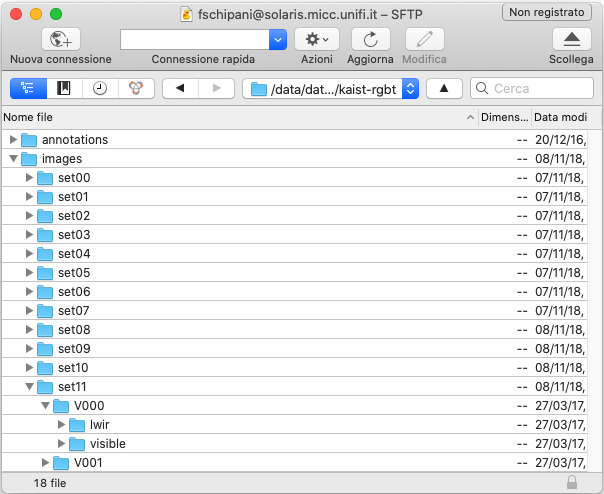
\includegraphics[width=0.7\textwidth]{images/screen_kaist.png}
    \caption{Suddivisione del dataset KAIST MPD}
    \label{fig:kaist_dataset_folder}
\end{figure} 
Il dataset in questione ha già una divisione predefinita tra train set e test set, ottenibile eseguendo uno script presente nella cartella del dataset. 

La successiva operazione che è stata effettuata è la stesura di un ulteriore script per convertire i suddetti file in un formato accettato dalla specifica implementazione di RetinaNet utilizzata, ovvero un \texttt{CSV} composto da colonne contenenti in ordine: il path dell'immagine, le eventuali coordinate della \ac{BB} e la classe di appartenenza della \ac{BB}. 

In questo dataset, come detto in Sezione \ref{subsec:kmpd}, sono presenti le classi \texttt{person}, \texttt{people}, \texttt{cyclist} e \texttt{person?}. A scopo di test sono state create due varianti dei file \texttt{CSV} poco sopra descritti. La prima variante comprende solamente le \ac{BB} che contengono \texttt{person} e \texttt{cyclist}, mentre la seconda variante, usata soprattutto in fase di test, comprende anche la classe \texttt{people} opportunamente rinominata alla necessità in \texttt{person}. Quest'ultima operazione è stata effettuata per far uniformare i label di due classi molto simili tra di loro in quanto per gli scopi degli esperimenti non è interessante il fatto che un pedone sia in gruppo, poco visibile o altro. L'importante è che compaia all'interno del frame. 
\paragraph{Annotazioni delle auto}
A differenza del dataset di FLIR, descritto in Sezione \ref{subsec:flirdataset}, qui mancano le annotazioni delle autovetture. Per effettuare altri esperimenti, descritti nelle sezioni a venire, è stato deciso di realizzarle a mano su $1000$ immagini. 

Al fine di rispecchiare il più possibile la divisione originale tra giorno e notte del dataset è stata necessaria un'analisi più approfondita della struttura stessa, da cui è derivato che sono presenti immagini diurne e notturne in numero molto simile. Per il dettaglio della suddivisione si può far riferimento a Tabella \ref{table:day_night_kaist}.
\begin{table}[]
    \begin{tabular}{c|cccccc}
    Diurne & SET00 & SET01 & SET02 & SET06 & SET07 & SET08 \\ \hline
    Notturne & SET03 & SET04 & SET05 & SET09 & SET10 & SET11
    \end{tabular}
    \caption{Suddivisione giorno notte di \ac{kmpd}}
    \label{table:day_night_kaist}
\end{table}
Sono state quindi selezionate casualmente $200$ immagini per ognuna delle cartelle \texttt{SET00/V000}, \texttt{SET05/V000}, \texttt{SET06/V001}, \texttt{SET08/V000} e \texttt{SET09/V000} e -- tramite lo strumento \ac{VIA} \cite{dutta2019vgg, dutta2016via} messo a disposizione gratuitamente -- sono state annotate tutte le auto, furgoni e bus non eccessivamente occlusi. 

Infine sono state prese le immagini di \texttt{SET00/V000} e \texttt{SET05/V000} per formare un piccolo train set, mentre quelle di \texttt{SET08/V000} e \texttt{SET09/V000} sono state usate per il test set. Il validation set è stato fatto con il \texttt{SET06/V001}. 

\subsection{FLIR Thermal Starter Dataset}
\label{subsec:flir_experiment}
Il dataset di FLIR ha richiesto molto poco preprocessing in quanto è stato sufficiente scrivere uno script che convertisse le annotazioni fornite con il dataset in un formato usabile da RetinaNet. In Codice \ref{code:flir_conversion} è possibile vedere il suddetto script. L'unica accortezza usata consiste nel selezionare solamente un sottoinsieme delle annotazioni, ovvero \texttt{people}, \texttt{bycicles} e \texttt{cars}. Questo è stato fatto per far coincidere il più possibile le annotazioni di questo dataset con quelle del dataset di Sezione \ref{subsec:kaist_experiment}.

\begin{lstlisting}[caption={Script di conversione per dataset FLIR}, language=Python, basicstyle=\tiny,label=code:flir_conversion]
import json
import glob
import csv
import itertools
import progressbar
if __name__ == "__main__":
    annotations_path = '/data/datasets/FLIR_ADAS/FLIR_ADAS/training/Annotations/*.json'
    id_to_name = {
        '1': 'People',
        '2': 'Bicycles',
        '3': 'Cars',
        '18': 'Dogs',
        '91': 'Other'
    }
    tot = len(glob.glob(annotations_path))
    bar = progressbar.ProgressBar(maxval=tot, widgets=[progressbar.Bar('=', '[', ']'), ' ', progressbar.Percentage()])
    i = 0
    bar.start()
    with open('thermal_validation_KAIST_TRAIN_WCARS.csv', 'w' ) as csvfile:
        filewriter = csv.writer(csvfile, delimiter=',', quotechar='|', quoting=csv.QUOTE_MINIMAL)
        for file_name in glob.iglob(annotations_path):
            data = json.load(open(file_name))
            if len(data['annotation'])>0:
                for i in range(len(data['annotation'])):
                    if data['annotation'][i]['category_id'] in ['1', '2', '3']:
                        x1, y1 = data['annotation'][i]['segmentation'][0][0],data['annotation'][i]['segmentation'][0][1]
                        x2, y2 = data['annotation'][i]['segmentation'][0][4],data['annotation'][i]['segmentation'][0][5]
                        filewriter.writerow([file_name.replace('Annotations', 'PreviewData')]+[x1, y1, x2, y2]+[id_to_name[data['annotation'][i]['category_id']]])
            else:
                filewriter.writerow([file_name, '',  '', '', '', ''])
            i = i+1
            bar.update(i)
    bar.finish()
  
\end{lstlisting}

\subsection{Video di Rete Ferroviaria Italiana}
\label{subsec:rfi_video_experiment}
I video termici forniti per il progetto di ricerca della tesi sono stati girati da telecamere \textit{Foshvision FS-UV535R104A Thermal Bi-spectrum} e \textit{HikVision DS-2TD2866-25 Thermal Bi-spectrum Network Bullet Camera} sul circuito di test di \ac{RFI} di San Donato a Bologna.
Il formato in cui sono stati forniti i video è \texttt{mp4}, quindi per renderli usabili da RetinaNet è stato reso necessario l'utilizzo del software \texttt{ffmpeg} per estrarre i singoli frame. 

Per realizzare una fase di fine tuning su tutti i layer della rete, analogamente a quello fatto in Sezione \ref{subsec:kaist_experiment}, sono stati annotati manualmente degli operai a lavoro su un unico video.
Il video in questione, della durata di circa $15$ minuti può essere segmentato in tre parti. La prima, che arriva circa fino al minuto $8$ non contiene alcun operaio o oggetto su cui è possibile realizzare annotazioni. La seconda parte, che inizia dal minuto 8 e si conclude quasi alla fine, vede degli operai che lavorano sulla linea ferroviaria. L'ultima parte è simile alla prima in quanto gli operai hanno finito il loro lavoro e non sono più nella scena ripresa dalla telecamera. 
Sempre come in Sezione \ref{subsec:kaist_experiment} sono state selezionate casualmente delle immagini. Dalla prima parte del video sono state selezionate $200$ immagini, dalla seconda $400$ e dall'ultima che è la più corta $100$. Le annotazioni anche in questo caso sono state realizzate con \ac{VIA}, solamente sulla seconda parte di video e solamente con la classe \texttt{person}.
 

\section{Esperimenti iniziali su immagini termiche}
\label{sec:init_experiment_thermal}
Riprendendo il discorso di Sezione \ref{sec:addestramento_iniziale_di_retinanet} si parlerà ora dei vari esperimenti effettuati con i vari dataset a disposizione. 




\paragraph{Test dei pesi di KAIST su FLIR}
L'obbiettivo di questa prima sperimentazione è consistito nel provare i risultati di Sezione \ref{subsec:rgb_to_thermal_kaist} sul dataset di FLIR. Il test è stato effettuato provando diverse soglie di rilevazione che variano tra $0.3$ a $0.8$ con passo di $0.1$. Il grafico di Figura \ref{fig:map_first_flir_lwir} riassume i risultati. 
\begin{figure}[]
    \centering
    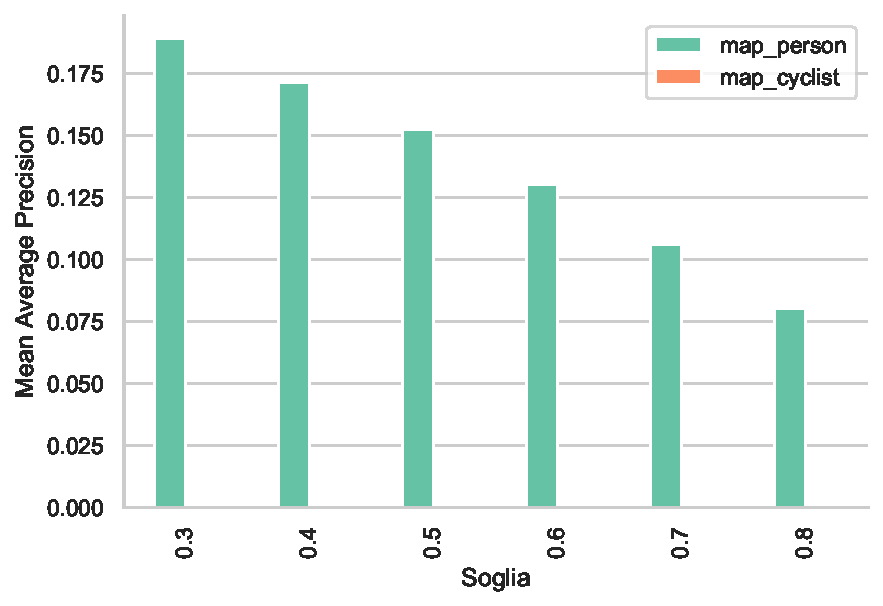
\includegraphics[width = 0.9\textwidth]{images/graphic/first_test_lwir_map.pdf}
    \caption{MAP al variare del valore di soglia su FLIR}
    \label{fig:map_first_flir_lwir}
\end{figure}
I risultati sono abbastanza deludenti, soprattutto sul fronte della rilevazione dei ciclisti. La motivazione principale è la carenza di esempi su quest'ultimi soprattutto se paragonati ai pedoni; un'altra motivazione degli scarsi risultati ottenuti è imputabile al diverso formato dell'annotazione in quanto su FLIR la \ac{BB} viene posta solamente sul ciclista, mentre su \ac{kmpd} sul ciclista più il mezzo. I risultati migliori comunque si ottengono con una soglia pari a $0.3$; in Figura \ref{fig:examples_first} mostriamo alcuni esempi di immagini annotate e classificate da RetinaNet, mentre in Tabella \ref{tab:first_experiment_flir} sono presenti i valori più dettagliati rispetto al miglior risultato. 
\begin{figure}[]
    \centering
    \makebox[\textwidth]{
    \subfloat{
        \begin{minipage}[b][][t]{.3\textwidth}
        \centering
        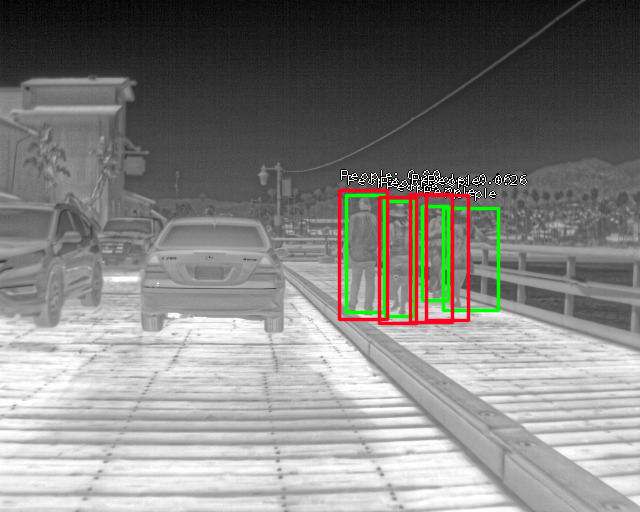
\includegraphics[width=.8\textwidth]{images/examples/first_flir_test/10.png}
        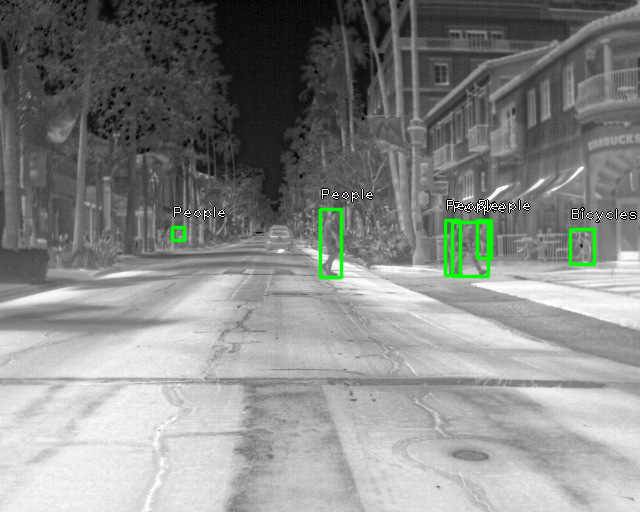
\includegraphics[width=.8\textwidth]{images/examples/first_flir_test/21.png}
        \end{minipage}
    }%
    \subfloat{
        \begin{minipage}[b][][t]{.3\textwidth}
        \centering
        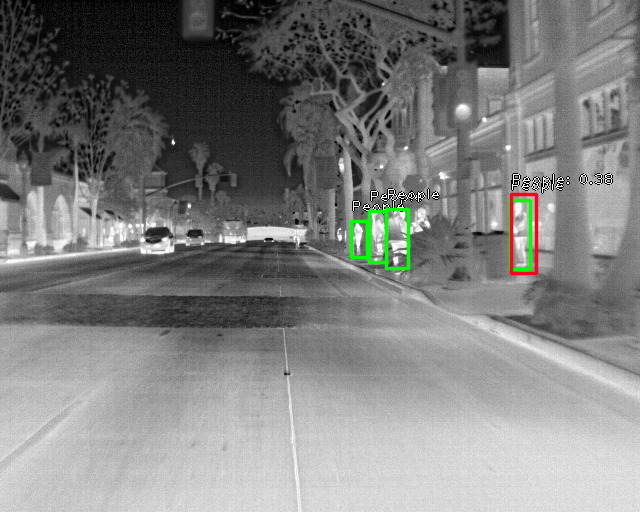
\includegraphics[width=.8\textwidth]{images/examples/first_flir_test/28.png}
        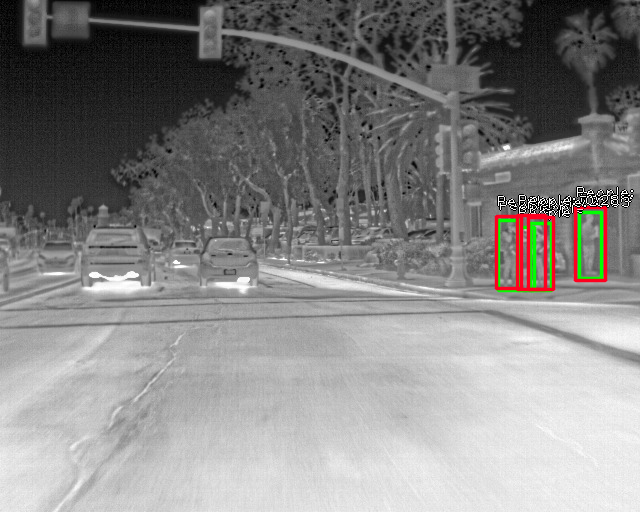
\includegraphics[width=.8\textwidth]{images/examples/first_flir_test/35.png}
        \end{minipage}
    }
    \subfloat{
        \begin{minipage}[b][][t]{.3\textwidth}
        \centering
        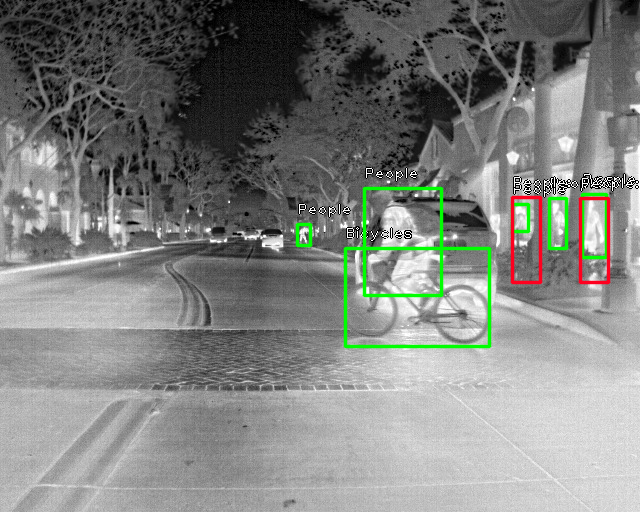
\includegraphics[width=.8\textwidth]{images/examples/first_flir_test/39.png}
        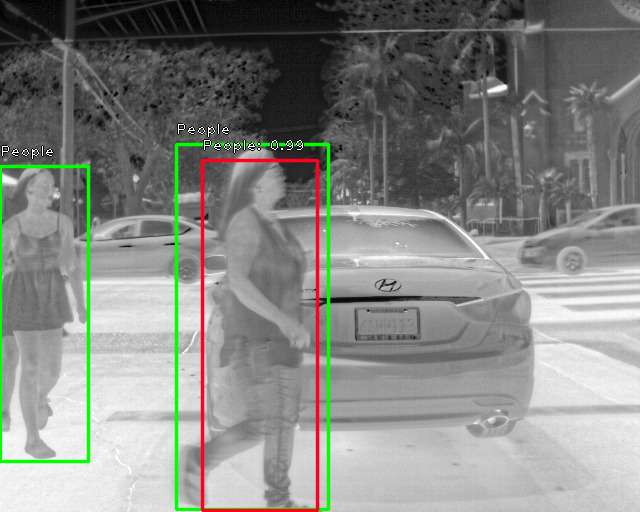
\includegraphics[width=.8\textwidth]{images/examples/first_flir_test/8.png}
        \end{minipage}
    }
    }
    \caption{Esempio di predizioni, in verde la \textit{ground truth} in rosso le predizioni.} 
    \label{fig:examples_first} 
\end{figure} 
\begin{table}[]
    \centering
    \begin{tabular}{c|c|c|}
    \cline{2-3}
     & Istanze & Map \\ \hline
    \multicolumn{1}{|c|}{Person} & 5779 & 0.1889 \\ \hline
    \multicolumn{1}{|c|}{Cyclist} & 471 & 0.0001 \\ \hline
    \multicolumn{1}{|c|}{Complessivo} & 6250 & 0.1747 \\ \hline
    \end{tabular}
    \caption{\ac{map} calcolata sul dataset FLIR partendo dai pesi di RetinaNet addestrato su \ac{kmpd} termico}
    \label{tab:first_experiment_flir}
\end{table}
La Figura \ref{fig:precision_recall_person_1} mostra la curva di precision-recall al variare della soglia di rilevamento, e si nota immediatamente una mancanza sia di precisione che di richiamo. Possiamo inoltre notare che se abbiamo maggior esempi classificati per via una soglia più bassa otteniamo una scarsa precisione sintomo che queste ultime rilevazioni sono in parte false; situazione contraria si verifica invece quando si aumenta la soglia di rilevamento con lo svantaggio però che in generale si ha una \textit{recall} minore.  
\begin{figure}[]
    \centering
    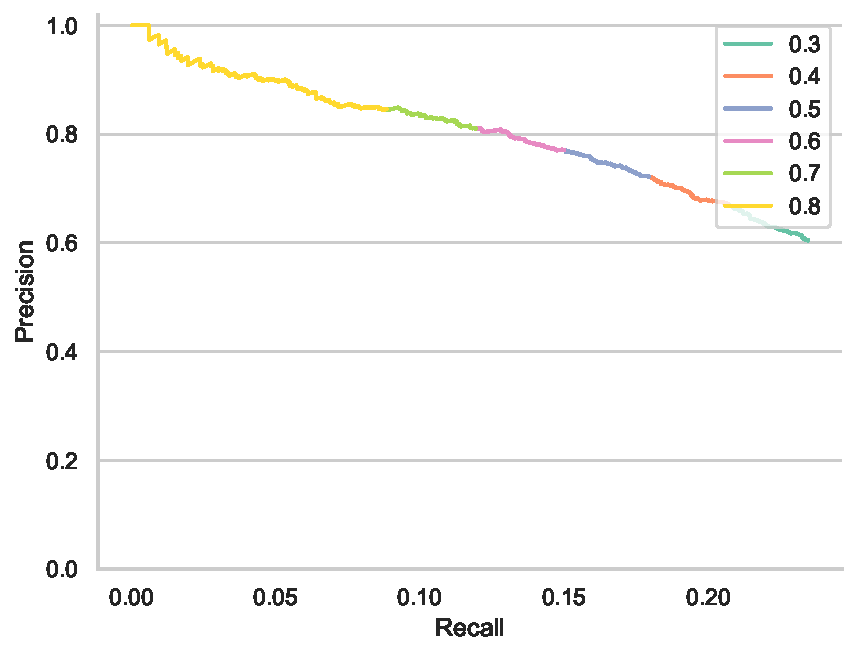
\includegraphics[width=\textwidth]{images/graphic/precision_recall_test_flir_kaist.pdf}
    \caption{Precision-Recall per classe \texttt{person}}
    \label{fig:precision_recall_person_1}
\end{figure}





\paragraph{Addestramento su FLIR partendo da COCO}
In questo esperimento si effettua una fase di addestramento di RetinaNet partendo dai pesi della rete preaddestrata sul dataset \ac{MSCOCO}. Dare questo tipo di imprinting al nostro modello permette di effettuare un'operazione considerabile alla stessa stregua del Transfer Learning, e di ridurre quindi sensibilmente i tempi di addestramento. 

Il grafico della fase di addestramento è in Figura \ref{fig:train_from_coco_FLIR} e mostra che le varie loss sono scese fino ad arrivare quasi a convergenza verso l'epoca $45$. La discesa è più stabile rispetto a quella vista in Sezione \ref{subsec:rgb_to_thermal_kaist} e questo è probabilmente dovuto alla migliore qualità di immagini di FLIR rispetto a \ac{kmpd}.  
\begin{figure}[]
    \centering
    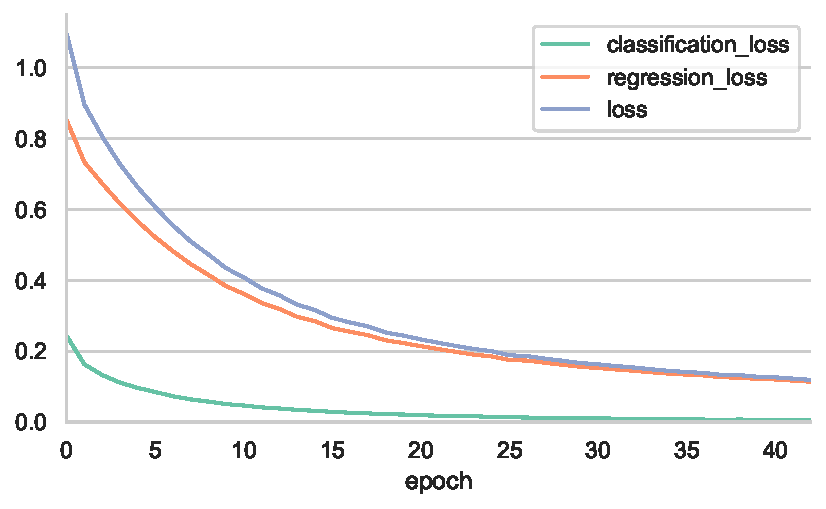
\includegraphics[width = \textwidth]{images/graphic/train_flir_from_coco.pdf}
    \caption{Addestramento di RetinaNet su FLIR partendo dai pesi di COCO}
    \label{fig:train_from_coco_FLIR}
\end{figure}

La fase di test inizialmente è stata effettuata solamente sul dataset di FLIR ottenendo i risultati in Figura \ref{fig:map_flir_from_coco}. 
\begin{figure}[]
    \centering
    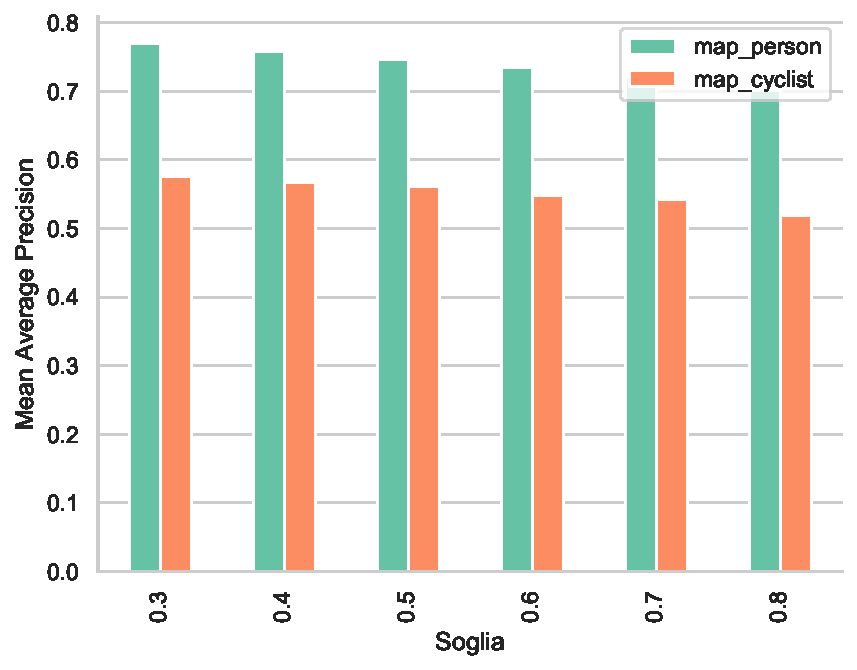
\includegraphics[width=\textwidth]{images/graphic/flir_from_coco_map.pdf}
    \caption{\ac{map} su FLIR addestrato dai pesi di COCO}
    \label{fig:map_flir_from_coco}
\end{figure}
Rispetto ai risultati mostrati in precedenza (Tabella \ref{tab:first_experiment_flir}) si ha un incremento notevole della \ac{map}. Come prima si verifica anche lo stesso fenomeno per cui si ottiene maggior \ac{map} con una soglia più bassa, ma a discapito della qualità delle rilevazioni. Si può osservare questo fenomeno guardando la curva di precision-recall in Figura \ref{fig:precision_recall_curve_flir_coco}. In Tabella \ref{table:coco_result_best_flir} sono presenti i risultati migliori ottenuti in termini di \ac{map}. 
\begin{figure}[]
    \centering
    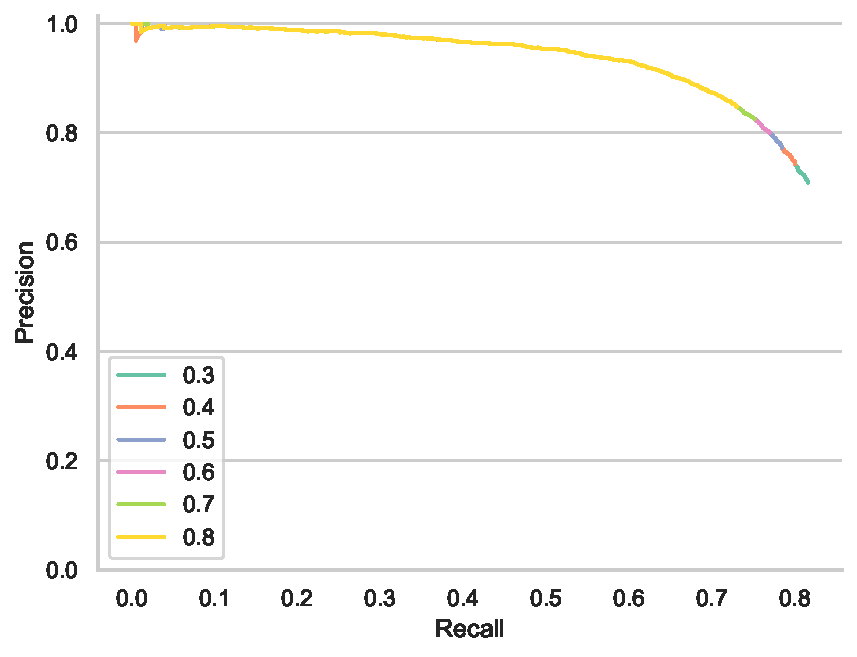
\includegraphics[width = \textwidth]{images/graphic/flir_coco_pr.pdf}
    \caption{Curva P/R di FLIR addestrato partendo da COCO (\texttt{person})}
    \label{fig:precision_recall_curve_flir_coco}
\end{figure}

\begin{table}[]
    \centering
    \begin{tabular}{c|c|c|}
    \cline{2-3}
     & Istanze & Map \\ \hline
    \multicolumn{1}{|c|}{Person} & 5779 & 0.575442 \\ \hline
    \multicolumn{1}{|c|}{Cyclist} & 471 & 0.769743 \\ \hline
    \multicolumn{1}{|c|}{Complessivo} & 6250 & 0.672592 \\ \hline
    \end{tabular}
    \caption{\ac{map} sul dataset FLIR dopo l'addestramento di RetinaNet partendo dai pesi del dataset \ac{MSCOCO}. Soglia di rilevamento pari a $0.3$.}
    \label{table:coco_result_best_flir}
\end{table}


\paragraph{Addestramento di FLIR partendo da KAIST}
Il fallimento del test in cui si testano i pesi di \ac{kmpd} sul dataset di FLIR è la ragione per cui occorre testare quest'ulteriore variante.

L'evoluzione delle misure di loss durante l'addestramento è visibile in Figura \ref{fig:flir_train_from_kaist}. Infatti ora si proverà ad addestrare sul dataset FLIR usando come base di partenza di RetinaNet i pesi derivanti dall'addestramento effettuato su \ac{kmpd}.

La prima cosa che si nota è l'andamento molto simile rispetto all'esperimento precedente, successivamente si può notare anche come si arriva ai medesimi risultati, ma con qualche epoca di anticipo. Infatti, nonostante i valori di partenza delle loss sono sensibilmente più elevati, si ha una discesa più repentina. Per quanto riguarda Precision/Recall e \ac{map} è possibile vedere grafici analoghi ai precedenti in Figura \ref{fig:flir_train_from_kaist_pr} e \ref{fig:flir_train_from_kaist_result}. L'andamento è comunque analogo al precedente ma, come si può vedere da Tabella \ref{table:best_flir_from_kaist}, si ottiene ovviamente un aumento della \ac{map} rispetto al test di Tabella \ref{tab:first_experiment_flir}, ma comunque si nota un calo delle performance rispetto a Tabella \ref{table:coco_result_best_flir}. Per maggiore chiarezza espositiva i risultati sono riassunti in Tabella \ref{tab:flir_comp}.
\begin{figure}[]
    \centering
    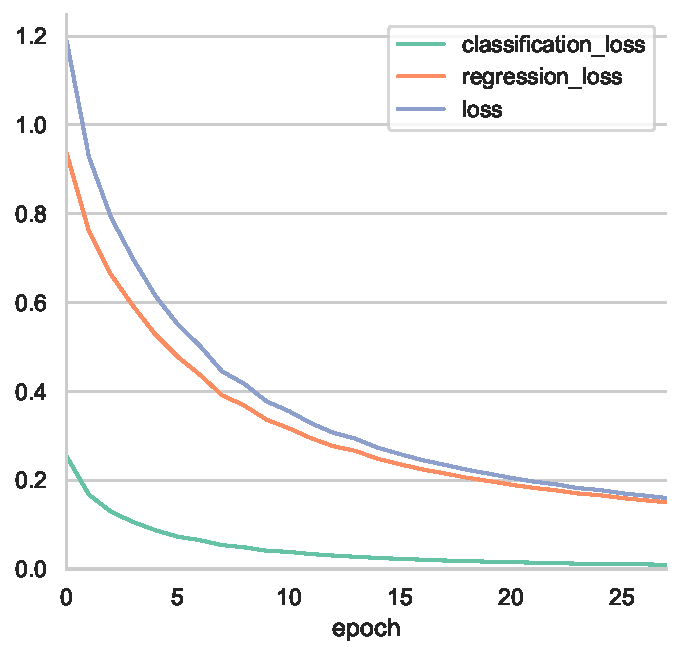
\includegraphics[width=0.9\textwidth]{images/graphic/flir_from_kaist.pdf}
    \caption{Addestramento su FLIR partendo dai pesi di KAIST}
    \label{fig:flir_train_from_kaist}
\end{figure}
\begin{figure}[]
    \centering
    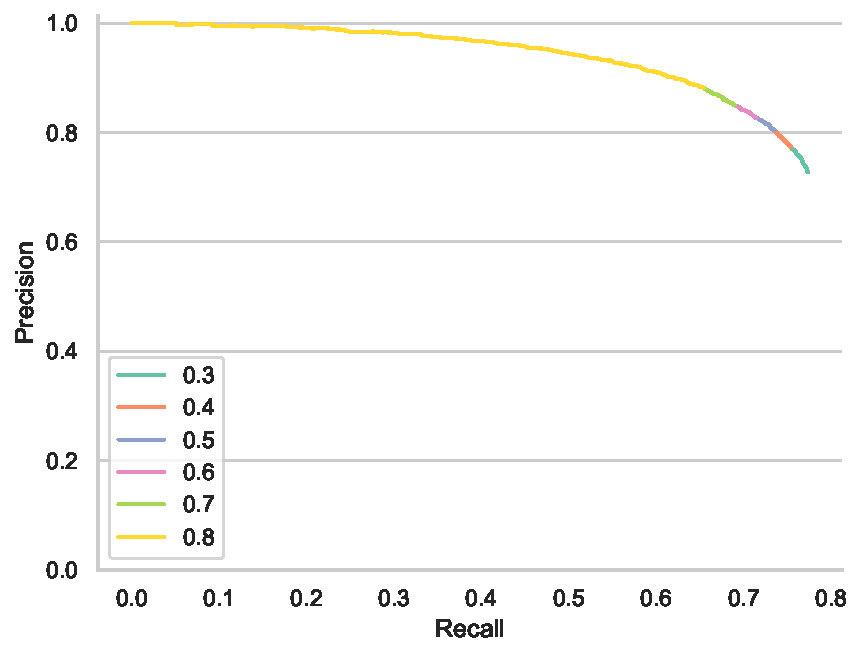
\includegraphics[width=0.9\textwidth]{images/graphic/flir_from_kaist_pr.pdf}
    \caption{Grafico P/R dell'addestramento su FLIR partendo dai pesi di KAIST (\texttt{person})}
    \label{fig:flir_train_from_kaist_pr}
\end{figure}
\begin{figure}[]
    \centering
    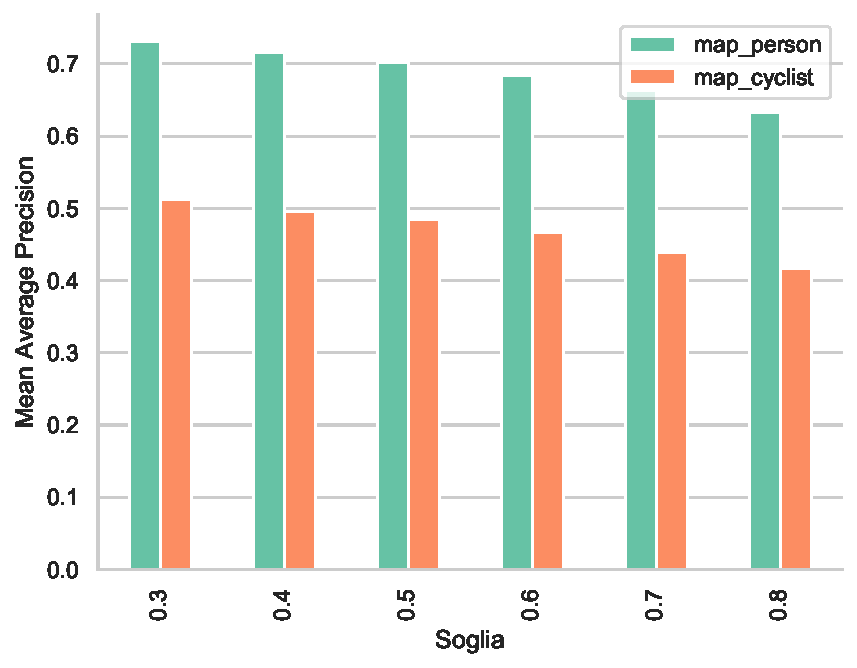
\includegraphics[width=0.9\textwidth]{images/graphic/flir_from_kaist_result.pdf}
    \caption{Risultati dell'addestramento su FLIR partendo dai pesi di KAIST}
    \label{fig:flir_train_from_kaist_result}
\end{figure}
\begin{table}[]
    \centering
    \begin{tabular}{c|c|c|}
    \cline{2-3}
     & Istanze & Map \\ \hline
    \multicolumn{1}{|c|}{Person} & 5779 & 0.512462 \\ \hline
    \multicolumn{1}{|c|}{Cyclist} & 471 & 0.730898 \\ \hline
    \multicolumn{1}{|c|}{Complessivo} & 6250 & 0.621680 \\ \hline
    \end{tabular}
    \caption{\ac{map} sul dataset FLIR dopo l'addestramento di RetinaNet partendo dai pesi precedenti ottenuti tramite train su \ac{kmpd}}
    \label{table:best_flir_from_kaist}
\end{table}

\begin{table}[]
    \resizebox{\textwidth}{!}{%
    \begin{tabular}{c|c|c|c|}
    \cline{2-4}
                                      & Da \ac{kmpd} & Da \ac{MSCOCO} & \textit{fine tuning} da \ac{kmpd} \\ \hline
    \multicolumn{1}{|c|}{Person}      & 0.1889   & 0.5754  & 0.5124        \\ \hline
    \multicolumn{1}{|c|}{Cyclist}     & 0.0001   & 0.7697  & 0.7308        \\ \hline
    \multicolumn{1}{|c|}{Complessivo} & 0.1747   & 0.6725  & 0.6216        \\ \hline
    \end{tabular}}
    \caption{Tabella riassuntiva dei risultati ottenuti tramite RetinaNet sul dataset di FLIR}
    \label{tab:flir_comp}
\end{table}

\paragraph{Test dei pesi migliori su KAIST} %FLIR_FROM_COCO_43.h5, imageSets/csv_files_NO_PEOPLE/lwir/test-night-01-no-people.csv, class_name_to_id_NO_PEOPLE.csv DESCRIVERE FIGURE
Per ora i pesi migliori ottenuti in termini di \ac{map} sulle persone è stato ottenuto addestrando RetinaNet sul dataset di FLIR partendo dai pesi della rete preaddestrata su \ac{MSCOCO}. Proviamo ora a vedere cosa succede testando questi pesi sul dataset di \ac{kmpd} in un caso che è già stato visto essere favorevole alla detection tramite immagini termiche, ovvero quando le acquisizioni sono state effettuate di notte.



\begin{figure}
    \begin{minipage}{.5\linewidth}
        \centering
        \subfloat[P/R su \texttt{person}]{
            \label{main:a}
            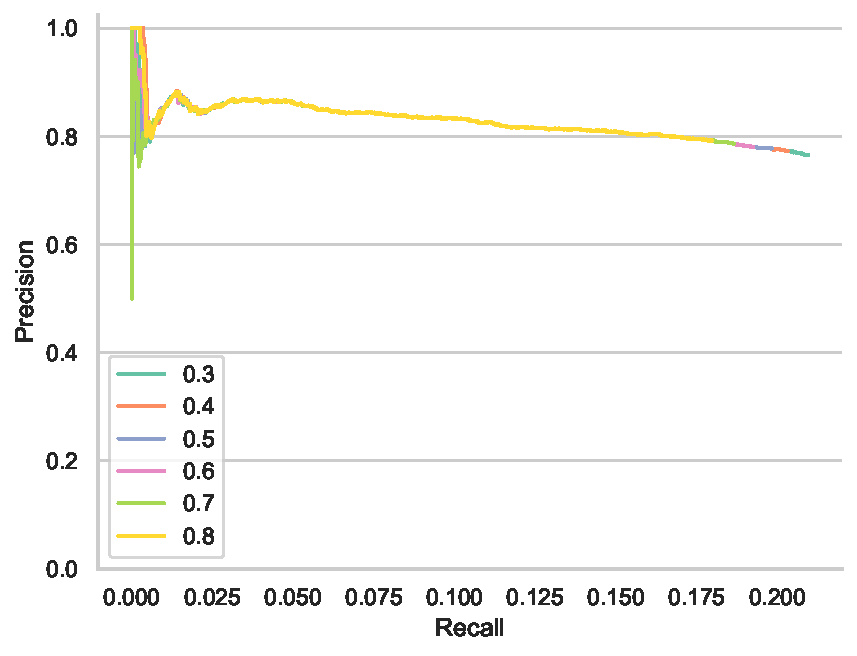
\includegraphics[scale=.5]{images/graphic/FLIR_FROM_COCO_PERSON.pdf}
        }
    \end{minipage}%
    \begin{minipage}{.5\linewidth}
        \centering
        \subfloat[\ac{map} su \texttt{person}]{
            \label{main:b}
            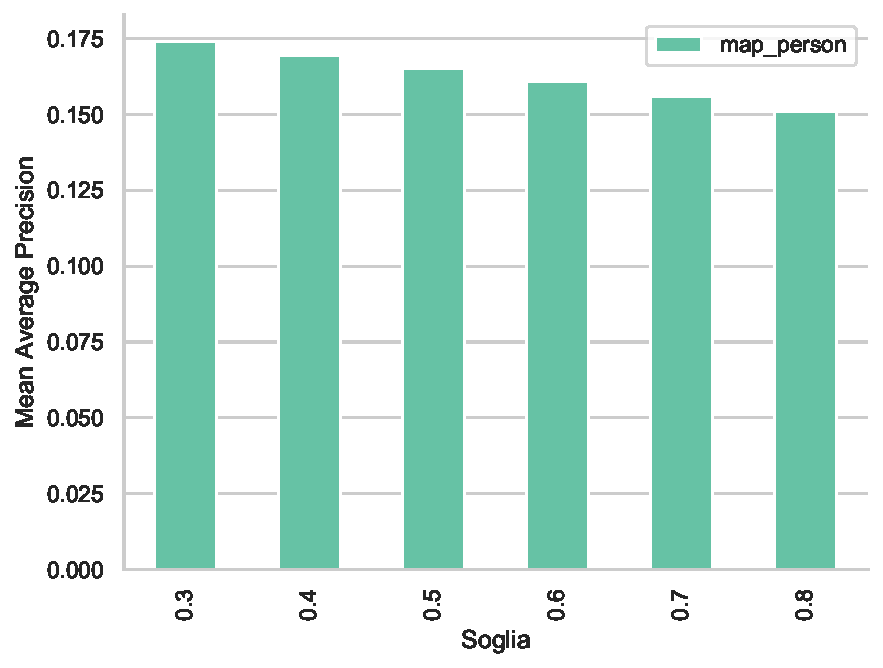
\includegraphics[scale=.5]{images/graphic/FLIR_FROM_COCO_RESULTS.pdf}
            }
    \end{minipage}
    \centering
    \caption{Test su KAIST del risultato migliore su FLIR}
    \label{fig:main}
\end{figure}

In Figura \ref{fig:main} è possibile visionare un sunto dei risultati ottenuti. Si può osservare in particolare nella parte \ref{main:b} che la \ac{map} ottenuta è molto bassa. Questa scarsa precisione in fase di inferenza porta a non avere grandi risultati all'atto pratico, basti vedere anche la Figura \ref{main:a} per notare come la curva di Precision/Recall indichi una forte penuria nella Recall. 
Dati alla mano si può dire sicuramente che le rilevazioni effettuate sono corrette, ma in pratica ne vengono trovate molte poche rispetto al totale. 

Infine riassumiamo in Tabella \ref{tab:best_kmpd_flir} i migliori risultati ottenuti per ora sulle persone e sui ciclisti all'interno dei vari dataset. 

\begin{table}[]
    \begin{tabular}{c|c|c|c|}
    \cline{2-4}
     & FLIR & \ac{kmpd} & \ac{kmpd} (Notte) \\ \hline
    \multicolumn{1}{|c|}{Person} & 0.5754 & 0.3415 & 0.4400 \\ \hline
    \multicolumn{1}{|c|}{Cyclist} & 0.7697 & 0.0387 & 0.0440 \\ \hline
    \multicolumn{1}{|c|}{Complessivo} & 0.6725 & 0.3353 & 0.4288 \\ \hline
    \end{tabular}
    \caption{Tabella riassuntiva delle migliori \ac{map} ottenute fino ad ora sui dataset di \ac{kmpd} termico e FLIR}
    \label{tab:best_kmpd_flir}
\end{table}

\subsection{Rilevazione delle auto} %riferimento in TODO -> "Per 5/10" DESCRIVERE ULTIME FIGURE
La rilevazione delle auto su entrambi i dataset ha richiesto un lavoro di preprocessing sul dataset \ac{kmpd} descritto in precedenza nella Sezione \ref{subsec:kaist_experiment}.
Il primo test effettuato consiste nel fissare una baseline data dall'addestramento su FLIR ed il secondo test si effettua sulla parte di dataset annotata manualmente di \ac{kmpd} cercando di vedere il comportamento con le autovetture. Il risultato è in Tabella \ref{table:baseline_car_kaist}. 
\begin{table}[]
    \centering
    \begin{tabular}{c|c|c|}
    \cline{2-3}
     & Istanze & Map \\ \hline
    \multicolumn{1}{|c|}{Person} & 755 & 0.3730 \\ \hline
    \multicolumn{1}{|c|}{Cyclist} & 15 & 0 \\ \hline
    \multicolumn{1}{|c|}{Cars} & 1088 & 0.5716 \\ \hline
    \multicolumn{1}{|c|}{Complessivo} & 6250 & 0.4863 \\ \hline
    \end{tabular}
    \caption{Baseline per la rilevazione di vetture su \ac{kmpd}. Test effettuato su \ac{kmpd} usando RetinaNet addestrata su FLIR.}
    \label{table:baseline_car_kaist}
\end{table} 

Il passo successivo è stata una fase di \textit{fine tuning} su tutta la rete di questi pesi sulla parte di train di \ac{kmpd} annotata manualmente con le vetture. Come si può vedere in Figura \ref{fig:fine_tuning_kaist_flir}, l'addestramento ha avuto una durata relativamente corta in quanto con solamente $15$ ore e $18$ epoche è arrivato al termine.
\begin{figure}[]
    \centering
    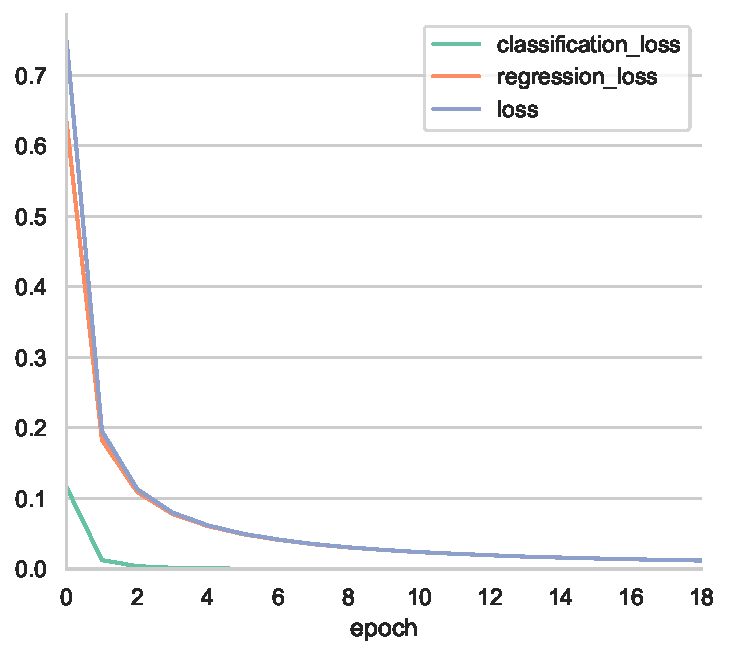
\includegraphics[width=\textwidth]{images/graphic/fine_tuning_kaist_flir.pdf}
    \caption{Fine tuning su tutta la rete usando \ac{kmpd} partendo da FLIR}
    \label{fig:fine_tuning_kaist_flir}
\end{figure}
Vista la repentina discesa delle loss e la scarsità di dati a disposizione è facile incorrere in un fenomeno di overfitting, ed infatti è quello che è accaduto. In Tabella \ref{tab:fine_tuning_kaist_flir} sono mostrati i risultati per alcune epoche di questa fase di addestramento, in grassetto ci sono i risultati migliori per ogni categoria. Come si può vedere nell'epoca $18$, ovvero l'ultima, non si raggiungono picchi di \ac{map}, il che è un sintomo di scarsa capacità di generalizzazione. Riguardo la classe \texttt{person} e \texttt{cyclist} il risultato migliore si ha all'epoca $8$. Invece riguardo la rilevazione di automobili si ha il risultato migliore all'epoca $10$. Si può notare inoltre che sia riguardo le persone che le automobili c'è stato un incremento nelle prestazioni della detection (Tabella \ref{tab:fine_tuning_kaist_flir_increment}). 
\begin{table}[]
    \centering
    \begin{tabular}{c|c|c|c|c|c|}
    \cline{2-6}
     & EP 18 & EP 10 & EP 09 & EP 08 & EP 05 \\ \hline
    \multicolumn{1}{|c|}{Person (755)} & 0.4964 & 0.5050 & 0.5018 & \textbf{0.5137} & 0.5048 \\ \hline
    \multicolumn{1}{|c|}{Cyclist (15)} & 0.0333 & 0.0444 & 0.0667 & \textbf{0.1000} & 0.0667 \\ \hline
    \multicolumn{1}{|c|}{Cars (1088)} & 0.6767 & \textbf{0.6929} & 0.6854 & 0.6787 & 0.6870 \\ \hline
    \multicolumn{1}{|c|}{Complessivo} & 0.5983 & \textbf{0.6113} & 0.6058 & 0.6070 & 0.6080 \\ \hline
    \end{tabular}
    \caption{Test di RetinaNet dopo il fine tuning di tutta la rete, partendo da FLIR, sulla parte di dataset di \ac{kmpd} annotato con le vetture. In grassetto i risultati migliori per classe. Tra parentesi il numero di istanze per classe.}
    \label{tab:fine_tuning_kaist_flir}
\end{table}
\begin{table}[]
    \centering
    \begin{tabular}{c|c|c|c|}
    \cline{2-4}
     & Post & Pre & Incremento \\ \hline
    \multicolumn{1}{|c|}{Person (755)} & 0.5137 & 0.3730 & +37\% \\ \hline
    \multicolumn{1}{|c|}{Cyclist (15)} & 0.1000 & 0.000 & + \\ \hline
    \multicolumn{1}{|c|}{Cars (1088)} & 0.6929 & 0.5716 & +21\% \\ \hline
    \multicolumn{1}{|c|}{Complessivo} & 0.6113 & 0.4863 & +25\% \\ \hline
    \end{tabular}
    \caption{Tabella riassuntiva dell'incremento ottenuto effettuando il fine tuning di rutta la rete da FLIR a \ac{kmpd}. Tra parentesi il numero di istanze per classe. }
    \label{tab:fine_tuning_kaist_flir_increment}
\end{table}

In particolare possiamo andare ad analizzare le performance ottenute all'epoca $10$ in quanto risultano mediamente le migliori. In Figura \ref{fig:test_kaist_ep8} sono presenti le curve di Precision/Recall sulla classe \texttt{person} e \texttt{cars}, mentre in Figura \ref{fig:test_kaist_ep8_map} sono presenti i grafici di \ac{map} al variare della soglia di rilevamento. Non è stata analizzata in maniera più dettagliata la classe \texttt{cyclist} in quanto gli esempi sono troppi pochi per ottenere risultati significativi. 

Andando a confrontare le curve di P/R di Figura \ref{fig:test_kaist_ep8} si nota come sulle automobili si hanno in media rilevazioni più precise ed anche un richiamo maggiore, il che porta ad avere detection sulle vetture in generale migliori rispetto a quelle ottenute sui pedoni. Il motivo presumibilmente può essere imputato ad una maggior somiglianza tra l'aspetto delle vetture in immagini termiche rispetto a quello che possono avere dei pedoni.  
\begin{figure}
    \begin{minipage}{.5\linewidth}
        \centering
        \subfloat[P/R su \texttt{person}]{
            \label{test_kaist_ep8:a}
            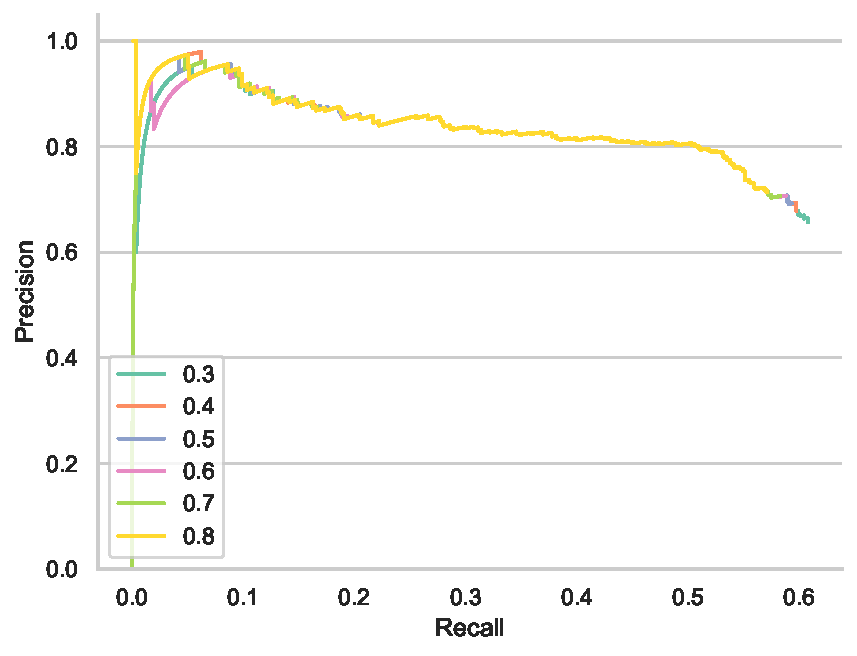
\includegraphics[scale=.5]{images/graphic/graphics_manual_annotations_08_person.pdf}
        }
    \end{minipage}%
    \begin{minipage}{.5\linewidth}
        \centering
        \subfloat[P/R su \texttt{cars}]{
            \label{test_kaist_ep8:b}
            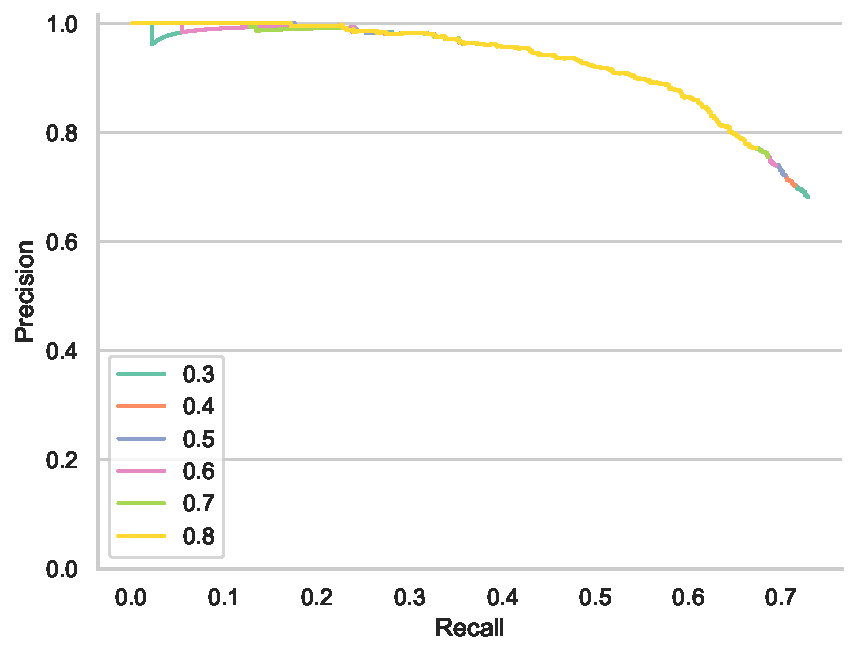
\includegraphics[scale=.5]{images/graphic/graphics_manual_annotations_08_cars.pdf}
            }
    \end{minipage}
    \centering
    \caption{P/R su KAIST all'epoca 10}
    \label{fig:test_kaist_ep8}
\end{figure}



\begin{figure}[]
    \centering
    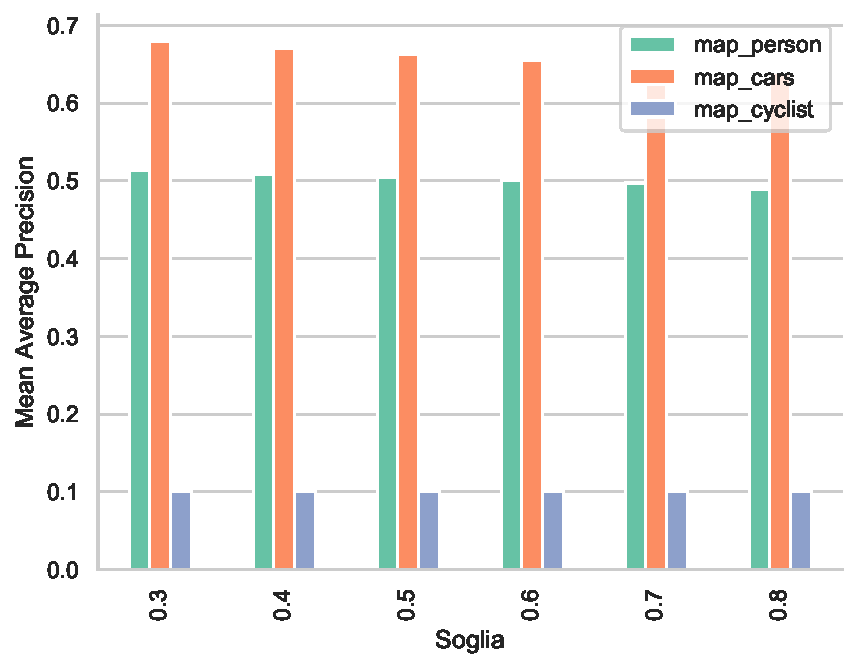
\includegraphics[width=\textwidth]{images/graphic/graphics_map.pdf}
    \caption{Fine tuning di KAIST partendo da FLIR}
    \label{fig:test_kaist_ep8_map}
\end{figure}

\section{Data Augmentation}
\label{sec:data_augmentaion_experiment}
Al fine di migliorare la qualità delle detection un ulteriore diramazione di esperimenti è stata svolta usando tecniche di Data Augmentation (Sezione \ref{sec:data_augmentation}). Le tecniche utilizzate in particolare sono AutoAugment, RandAugment ed infine delle immagini termiche generate da una \ac{GAN}. L'utilizzo di queste tecniche è motivato dal fatto che, soprattutto nella parte di dataset di \ac{kmpd} annotata manualmente, le annotazioni sono poco numerose. Quindi si prova ad aumentarne virtualmente il loro numero variandone l'aspetto tramite trasformazioni sull'immagine o porzioni di essa.
\paragraph{AutoAugment}
AutoAugment richiede un'elevata richiesta computazionale, che non è alla portata dell'hardware utilizzato per lo sviluppo della tesi, quindi non è stato sfruttato adeguatamente, bensì sono state usate policy derivanti dagli addestramenti effettuati su altri dataset. 
In Codice \ref{code:policy_v0}, \ref{code:policy_v1} e \ref{code:policy_v2} sono presenti le tre politiche di AutoAugment con cui sono stati effettuati gli esperimenti.  

\begin{lstlisting}[caption={Policy V0 di AutoAugment}, language=Python, basicstyle=\tiny,label=code:policy_v0]
def policy_v0():
  policy = [
      [('TranslateX_BBox', 0.6, 4), ('Equalize', 0.8, 10)],
      [('TranslateY_Only_BBoxes', 0.2, 2), ('Cutout', 0.8, 8)],
      [('Sharpness', 0.0, 8), ('ShearX_BBox', 0.4, 0)],
      [('ShearY_BBox', 1.0, 2), ('TranslateY_Only_BBoxes', 0.6, 6)],
      [('Rotate_BBox', 0.6, 10), ('Color', 1.0, 6)],
  ]
  return policy
\end{lstlisting}
La prima policy è la più semplice tra le tre, contiene al suo interno solamente cinque subpolicy formate a loro volta da due operazioni.
\begin{lstlisting}[caption={Policy V1 di AutoAugment}, language=Python, basicstyle=\tiny,label=code:policy_v1]
def policy_v1():
    policy = [
        [('TranslateX_BBox', 0.6, 4), ('Equalize', 0.8, 10)],
        [('TranslateY_Only_BBoxes', 0.2, 2), ('Cutout', 0.8, 8)],
        [('Sharpness', 0.0, 8), ('ShearX_BBox', 0.4, 0)],
        [('ShearY_BBox', 1.0, 2), ('TranslateY_Only_BBoxes', 0.6, 6)],
        [('Rotate_BBox', 0.6, 10), ('Color', 1.0, 6)],
        [('Color', 0.0, 0), ('ShearX_Only_BBoxes', 0.8, 4)],
        [('ShearY_Only_BBoxes', 0.8, 2), ('Flip_Only_BBoxes', 0.0, 10)],
        [('Equalize', 0.6, 10), ('TranslateX_BBox', 0.2, 2)],
        [('Color', 1.0, 10), ('TranslateY_Only_BBoxes', 0.4, 6)],
        [('Rotate_BBox', 0.8, 10), ('Contrast', 0.0, 10)],
        [('Cutout', 0.2, 2), ('Brightness', 0.8, 10)],
        [('Color', 1.0, 6), ('Equalize', 1.0, 2)],
        [('Cutout_Only_BBoxes', 0.4, 6), ('TranslateY_Only_BBoxes', 0.8, 2)],
        [('Color', 0.2, 8), ('Rotate_BBox', 0.8, 10)],
        [('Sharpness', 0.4, 4), ('TranslateY_Only_BBoxes', 0.0, 4)],
        [('Sharpness', 1.0, 4), ('SolarizeAdd', 0.4, 4)],
        [('Rotate_BBox', 1.0, 8), ('Sharpness', 0.2, 8)],
        [('ShearY_BBox', 0.6, 10), ('Equalize_Only_BBoxes', 0.6, 8)],
        [('ShearX_BBox', 0.2, 6), ('TranslateY_Only_BBoxes', 0.2, 10)],
        [('SolarizeAdd', 0.6, 8), ('Brightness', 0.8, 10)],
    ]
    return policy
\end{lstlisting}
La seconda, a differenza della prima, introduce un numero di subpolicy più alto, ma mantiene il numero di operazioni applicabili ad immagine. 

\begin{lstlisting}[caption={Policy V2 di AutoAugment}, language=Python, basicstyle=\tiny,label=code:policy_v2]
def policy_v2():
    policy = [
        [('Color', 0.0, 6), ('Cutout', 0.6, 8), ('Sharpness', 0.4, 8)],
        [('Rotate_BBox', 0.4, 8), ('Sharpness', 0.4, 2),
         ('Rotate_BBox', 0.8, 10)],
        [('TranslateY_BBox', 1.0, 8), ('AutoContrast', 0.8, 2)],
        [('AutoContrast', 0.4, 6), ('ShearX_BBox', 0.8, 8),
         ('Brightness', 0.0, 10)],
        [('SolarizeAdd', 0.2, 6), ('Contrast', 0.0, 10),
         ('AutoContrast', 0.6, 0)],
        [('Cutout', 0.2, 0), ('Solarize', 0.8, 8), ('Color', 1.0, 4)],
        [('TranslateY_BBox', 0.0, 4), ('Equalize', 0.6, 8),
         ('Solarize', 0.0, 10)],
        [('TranslateY_BBox', 0.2, 2), ('ShearY_BBox', 0.8, 8),
         ('Rotate_BBox', 0.8, 8)],
        [('Cutout', 0.8, 8), ('Brightness', 0.8, 8), ('Cutout', 0.2, 2)],
        [('Color', 0.8, 4), ('TranslateY_BBox', 1.0, 6), ('Rotate_BBox', 0.6, 6)],
        [('Rotate_BBox', 0.6, 10), ('BBox_Cutout', 1.0, 4), ('Cutout', 0.2, 8)],
        [('Rotate_BBox', 0.0, 0), ('Equalize', 0.6, 6), ('ShearY_BBox', 0.6, 8)],
        [('Brightness', 0.8, 8), ('AutoContrast', 0.4, 2),
         ('Brightness', 0.2, 2)],
        [('TranslateY_BBox', 0.4, 8), ('Solarize', 0.4, 6),
         ('SolarizeAdd', 0.2, 10)],
        [('Contrast', 1.0, 10), ('SolarizeAdd', 0.2, 8), ('Equalize', 0.2, 4)],
    ]
    return policy
  
\end{lstlisting}
La terza invece diminuisce leggermente il numero di subpolicy rispetto alla seconda, ma aumenta le operazioni applicabili ad immagine a 3. 

Le seguenti politiche sono state usate per addestrare RetinaNet sulla parte di dataset di \ac{kmpd} con i label sulle vetture. 

Effettuando tre diverse fasi di addestramento ognuna con una policy diversa si ottengono in fase di inferenza i risultati riassunti in Tabella \ref{table:aa_kaist}. Rispetto ai risultati ottenuti in precedenza si ha un miglioramento nella rilevazione delle automobili usando la policy V0 all'epoca 5, mentre per i pedoni si ha un miglioramento nella rilevazione usando la politica V2 sempre all'epoca 5. Le variazioni tra i risultati migliori ottenuti in precedenza e quelli migliori ottenuti con AutoAugment sono riassunti in Tabella \ref{table:AA_increment}.

\begin{table}[]
    \centering
    \resizebox{\textwidth}{!}{%
    \begin{tabular}{|c|c|c|c|c|c|c|c|c|c|c|c|c|c|c|c|}
        \hline
        Policy & V0 & V0 & V0 & V1 & V1 & V1 & V1 & V1 & V1 & V2 & V2 & V2 & V2 & V2 & V2 \\ \hline
        Epoca & 5 & 8 & 11 & 5 & 10 & 15 & 20 & 30 & 33 & 05 & 10 & 15 & 20 & 30 & 37 \\ \hline
        Person (755) & 0.4808 & 0.4850 & 0.4982 & 0.5157 & 0.5005 & 0.4896 & 0.4876 & 0.4975 & 0.3873 & \cellcolor[HTML]{9AFF99}\textbf{0.5241} & 0.5032 & 0.5007 & 0.4959 & 0.5064 & 0.5064 \\ \hline
        Cyclist (15) & 0.0067 & \cellcolor[HTML]{9AFF99}\textbf{0.0167} & 0.0000 & 0.0000 & 0.0000 & 0.0000 & 0.0000 & 0.0000 & 0.0000 & 0.0000 & 0.0000 & 0.0000 & 0.0000 & 0.0000 & 0.0000 \\ \hline
        Cars (1088) & \cellcolor[HTML]{9AFF99}\textbf{0.7195} & 0.6942 & 0.6792 & 0.6805 & 0.6728 & 0.6605 & 0.6703 & 0.6693 & 0.5603 & 0.6506 & 0.6564 & 0.6505 & 0.6254 & 0.6264 & 0.6265 \\ \hline
        Complessivo & \cellcolor[HTML]{9AFF99}\textbf{0.6167} & 0.6037 & 0.6002 & 0.6080 & 0.5973 & 0.5857 & 0.5906 & 0.5941 & 0.4855 & 0.5940 & 0.5888 & 0.5844 & 0.5677 & 0.5726 & 0.5726 \\ \hline
        \end{tabular}}
    \caption{\ac{map} ottenute tramite l'utilizzo delle varie policy predefinite di AutoAugment sul dataset di \ac{kmpd}. La base di partenza sono i migliori risultati ottenuti fino ad ora sulla parte di dataset di \ac{kmpd} con le annotazioni sulle vetture.}
    \label{table:aa_kaist}
\end{table}


\begin{table}[]
    \centering
    \begin{tabular}{c|c|c|c|}
    \cline{2-4}
     & Prima di AA & Dopo AA & Variazione \\ \hline
    \multicolumn{1}{|c|}{Person (755)} & 0.5137 & 0.5241 & +2\% \\ \hline
    \multicolumn{1}{|c|}{Cyclist (15)} & 0.1000 & 0.0167 & -0.4\%\\ \hline
    \multicolumn{1}{|c|}{Cars (1088)} & 0.6929 & 0.7195 & +3.8\% \\ \hline
    \multicolumn{1}{|c|}{Complessivo} & 0.6113 & 0.6167 & +0.8\% \\ \hline
    \end{tabular}
    \caption{Variazioni rispetto alla baseline dopo l'utilizzo di AutoAugment sul dataset di \ac{kmpd} con le annotazioni sulle vetture.}
    \label{table:AA_increment}
\end{table}

Un ulteriore esperimento effettuato con AutoAugment è relativo al miglioramento della rilevazione dei pedoni. In pratica è stata usata la politica che ha fatto ottenere un miglioramento nella rilevazione dei pedoni per effettuare un training sul dataset di FLIR. Lo scopo era di ottenere miglior capacità di generalizzazione e quindi passare da un dataset all'altro con risultati migliori. In Tabella \ref{table:tl_flir_kaist_aav2} sono presenti i risultati dell'esperimento appena descritto, mentre in Figura \ref{fig:AA_v2} è presente il grafico riguardante la progressione delle Loss durante la fase di addestramento. 
\begin{figure}[]
    \centering
    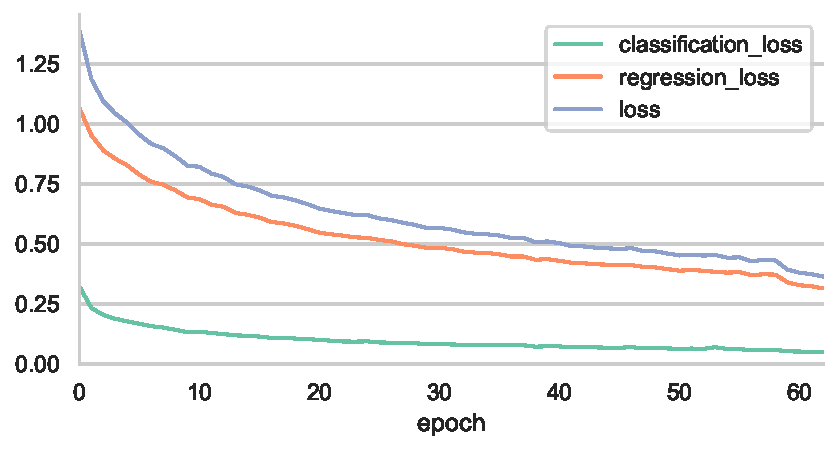
\includegraphics[width=\textwidth]{images/graphic/train_aa_flir_v2.pdf}
    \caption{Training su FLIR con policy di AutoAugment V2}
    \label{fig:AA_v2}
\end{figure}

\begin{table}[]
    \begin{tabular}{c|c|c|c|c|c|c|}
    \cline{2-7}
     & EP 05 & EP 20 & EP 20 & EP 50 & EP 63 & NO AA\\ \hline
    \multicolumn{1}{|c|}{Person (755)} & 0.3342 & 0.2516 & 0.3619 & 0.3270 & 0.3531 & 0.3730 \\ \hline
    \end{tabular}
    \caption{Risultati del test su \ac{kmpd} usando RetinaNet addestrato con e senza la policy di AutoAugment V2 sul dataset di FLIR.}
    \label{table:tl_flir_kaist_aav2}
\end{table}

L'ultimo esperimento effettuato con AutoAugment parte dai pesi di quello precedentemente descritto (Figura \ref{fig:AA_v2}, Tabella \ref{table:tl_flir_kaist_aav2}) realizzando una fase di \textit{fine tuning} di tutti i layer della rete sul dataset di KAIST. In Tabella \ref{table:fine_tuning_aav2_kaist} sono presenti i risultati di questa ultima fase, e come si può vedere non si ottiene alcun miglioramento. 

\begin{table}[]
    \resizebox{\textwidth}{!}{%
    \begin{tabular}{c|c|c|c|c|c|c|c|c|c|}
    \cline{2-10}
     & EP 05 & EP 10 & EP 15 & EP 20 & EP 25 & EP 30 & EP 35 & EP 40 & EP 44 \\ \hline
    \multicolumn{1}{|c|}{Person (755)} & 0.5061 & 0.4899 & 0.4913 & 0.4959 & 0.4822 & 0.4847 & 0.5035 & 0.4859 & 0.4911 \\ \hline
    \multicolumn{1}{|c|}{Cyclist (15)} & 0.0000 & 0.0000 & 0.0000 & 0.0000 & 0.0000 & 0.0000 & 0.0000 & 0.0000 & 0.0000 \\ \hline
    \multicolumn{1}{|c|}{Cars (1088)} & 0.5250 & 0.5395 & 0.5360 & 0.5383 & 0.5462 & 0.5427 & 0.5454 & 0.5387 & 0.5399 \\ \hline
    \multicolumn{1}{|c|}{Complessivo} & 0.5131 & 0.5150 & 0.5135 & 0.5167 & 0.5158 & 0.5148 & 0.5239 & 0.5129 & 0.5157 \\ \hline
    \end{tabular}}
    \caption{Test di RetinaNet su \ac{kmpd} dopo un fine tuning partendo dai pesi del precedente addestramento realizzato su FLIR con AutoAugment V2.}
    \label{table:fine_tuning_aav2_kaist}
\end{table}

\paragraph{RandAugment} 
RandAugment, come precedentemente descritto in Sezione \ref{subsec:rand_augment}, riduce notevolmente il costo computazionale rispetto ad AutoAugment per far sì che si adatti al dataset su cui sarà applicato. 

In questo caso si hanno solo due parametri $N$ ed $M$, con il primo che indica il numero di operazioni da applicare, ed il secondo la potenza con cui applicarle. Ci si riconduce in breve ad un problema di ottimizzazione di iperparametri risolvibile anche con un algoritmo GridSearch. In questa tesi però è stata usata la piattaforma \href{http://www.comet.ml}{Comet.ml} che implementa una serie di algoritmi per realizzare ottimizzazione. L'algoritmo scelto è stato quello che la piattaforma definisce il migliore, un algoritmo di tipo \textit{bayesiano} su cui non vengono rilasciati ulteriori dettagli.

Il target dell'ottimizzatore è la minimizzazione della \ac{map} complessiva moltiplicata per $-1$, in pratica quindi è la massimizzazione della metrica. L'intero processo ha avuto una durata di circa $130$ ore consecutive in quanto l'ambiente è stato impostato per eseguire una fase di training di $7$ epoche seguita da un test per la valutazione delle performance, partendo dai pesi di RetinaNet preaddestrata su \ac{MSCOCO}. Il tutto è stato realizzato sulla parte di dataset di \ac{kmpd} con le annotazioni delle automobili. Un sommario dell'ottimizzazione è in Figura \ref{fig:map_comet_ml} e come si può vedere i risultati migliori si ottengono ponendo $M$ con valori compresi tra $26$ e $30$ e con $N$ uguale a $3$.
\begin{figure}[]
    \centering
    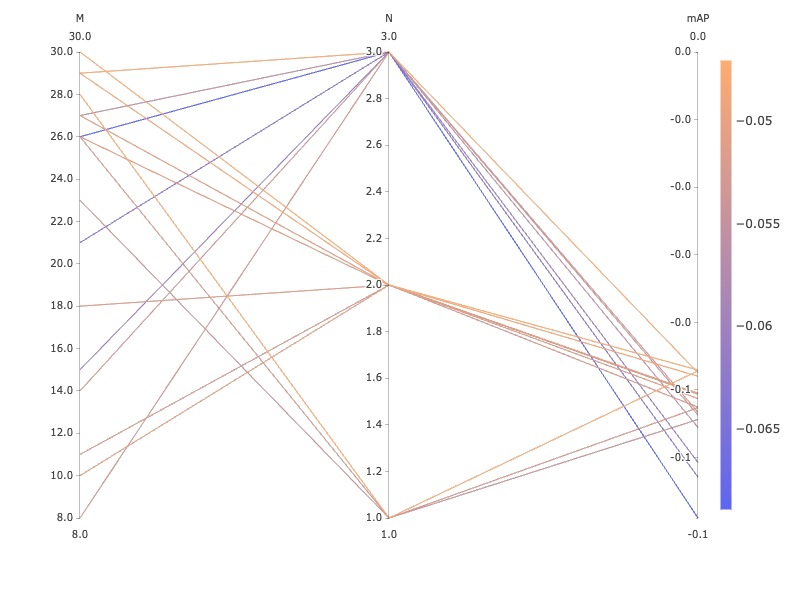
\includegraphics[width=0.9\textwidth]{images/graphic/mAP_comet.jpeg}
    \caption{\ac{map} al variare degli iperparametri durante l'ottimizzazione di RandAugment usando come target la \ac{map} complessiva ottenuta sul dataset \ac{kmpd}}
    \label{fig:map_comet_ml}
\end{figure}

Purtroppo questa ottimizzazione però non ha portato a miglioramenti probabilmente perché sette epoche non sono sufficienti partendo da pesi generici come quelli di \ac{MSCOCO}. Si ottiene una \ac{map} sulle persone pari a $0.4769$, mentre per le vetture si arriva a $0.6646$. 

Con RandAugment è stato effettuato un ulteriore esperimento per verificare se effettivamente un tipo di augmentation del genere potesse portare a migliorare dei risultati già ottenuti. A partire dai risultati di Tabella \ref{tab:fine_tuning_kaist_flir} l'esperimento effettuato ha avuto come target il miglioramento della \ac{map} sulla classe \texttt{person}. 
È stato quindi lanciato nuovamente l'ottimizzatore di iperparametri, ma a differenza di prima la base di partenza non è \ac{MSCOCO} bensì i pesi di RetinaNet all'ottava epoca di Tabella \ref{tab:fine_tuning_kaist_flir}. 

\begin{figure}[]
    \begin{minipage}{.5\linewidth}
        \centering
        \subfloat[\ac{map}]{
            \label{RA_2:a}
            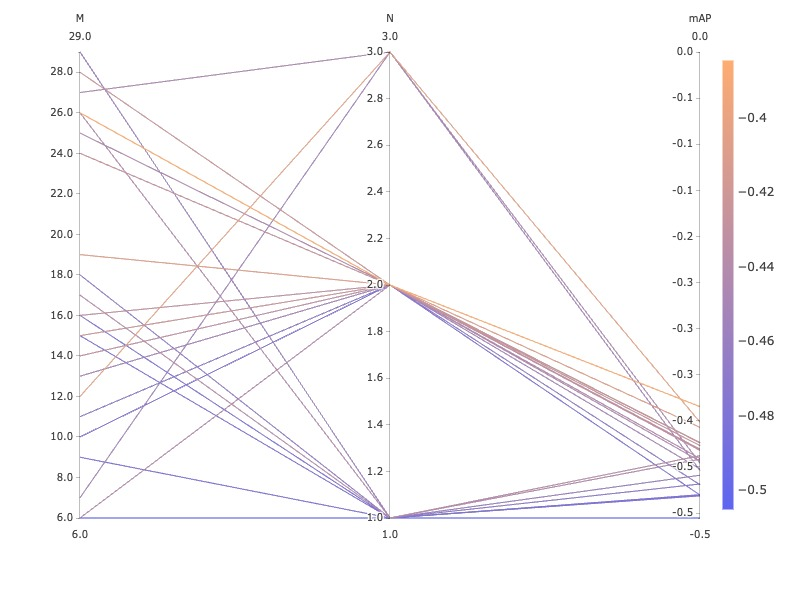
\includegraphics[width =0.90\textwidth]{images/graphic/mAP_person_RA.jpeg}
        }
    \end{minipage}%
    \begin{minipage}{.5\linewidth}
        \centering
        \subfloat[Validation loss]{
            \label{RA_2:b}
            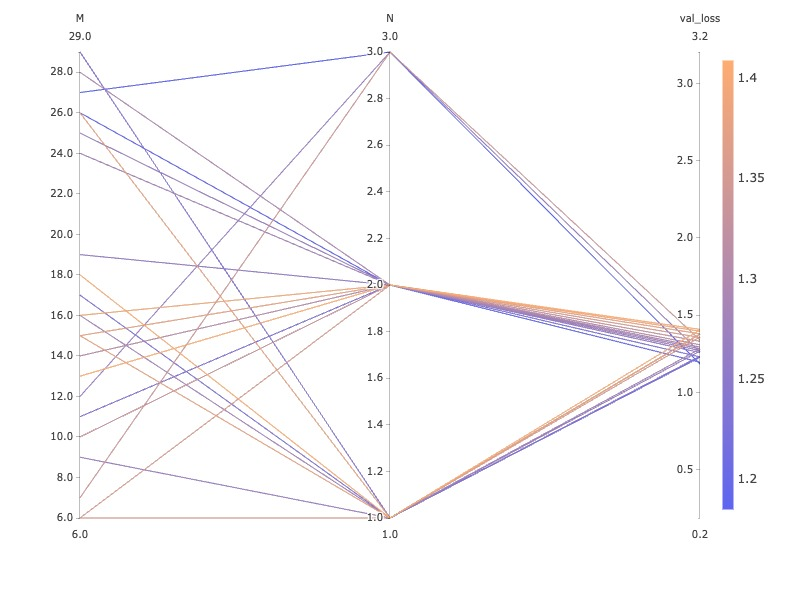
\includegraphics[width = 0.90\textwidth]{images/graphic/val_loss_person_RA.jpeg}
            }
    \end{minipage}
    \centering
    \caption{Andamento del processo di ottimizzazione di RandAugment sulla classe \texttt{person}}
    \label{fig:RA_2}
\end{figure}

Rispetto alla prima fase di ottimizzazione i risultati possono essere considerati diametralmente opposti in quanto, come è possibile vedere da Figura \ref{RA_2:a}, si ottiene maggior \ac{map} per parametri di \textit{RandAugment} decisamente più blandi. In particolare il risultato migliore si ottiene ponendo $M$ uguale a $6$ ed $N$ uguale ad $1$.
Dopo questa nuova fase di ricerca di iperparametri è stata effettuata una nuova fase di addestramento di RetinaNet per vedere a che risultati portasse.
\begin{figure}[]
    \centering
    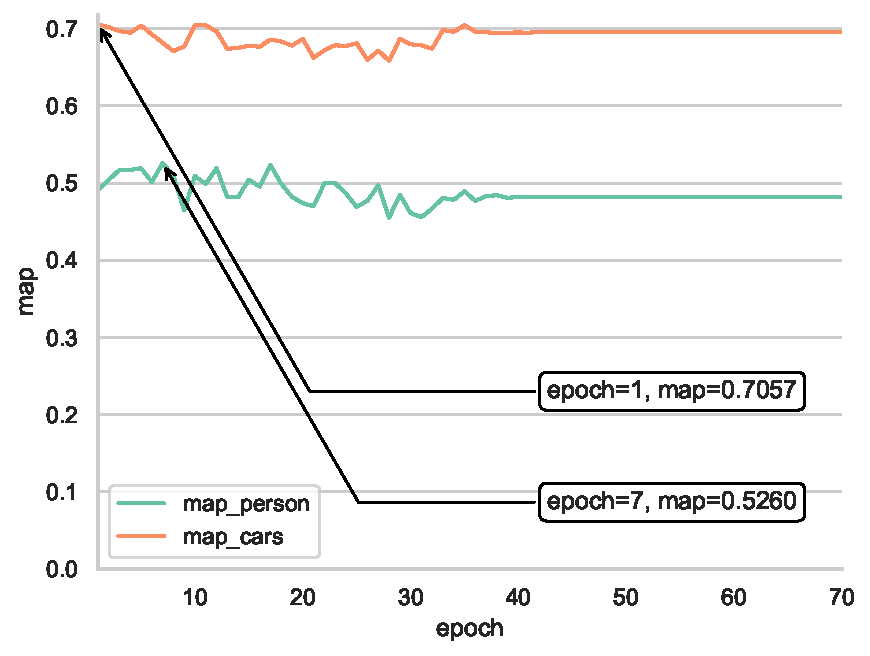
\includegraphics[width=\textwidth]{images/graphic/map_person_ra.pdf}
    \caption{Risultati ottenuti su \ac{kmpd} tramite l'ottimizzazione specifica di RandAugment su \texttt{person}}
    \label{fig:ra_person}
\end{figure}

Ciò che è stato ottenuto da questo esperimento è verificabile in Figura \ref{fig:ra_person} e mette alla luce come con \textit{RandAugment} si possano ottenere prestazioni del tutto paragonabili ad \textit{AutoAugment} con un computo decisamente più breve e gestibile. Infatti la massima \ac{map} ottenuta eseguendo una specifica ottimizzazione su \texttt{person}, è anche leggermente superiore a quello che è stato ottenuto usando delle policy predefinite su \textit{AutoAugment}.

Lo stesso esperimento è stato ripetuto utilizzando come target dell'ottimizzazione la \ac{map} sulla classe \texttt{cars}. I risultati ottenuti sono visibili in Figura \ref{fig:RA_3}.
L'andamento è del tutto similare a quanto ottenuto con l'ottimizzazione effettuata con la classe \texttt{person}, non ottenendo però alcun miglioramento in termini di \ac{map} su nessuna delle classi.

\begin{figure}[]
    \begin{minipage}{.5\linewidth}
        \centering
        \subfloat[\ac{map}]{
            \label{RA_3:a}
            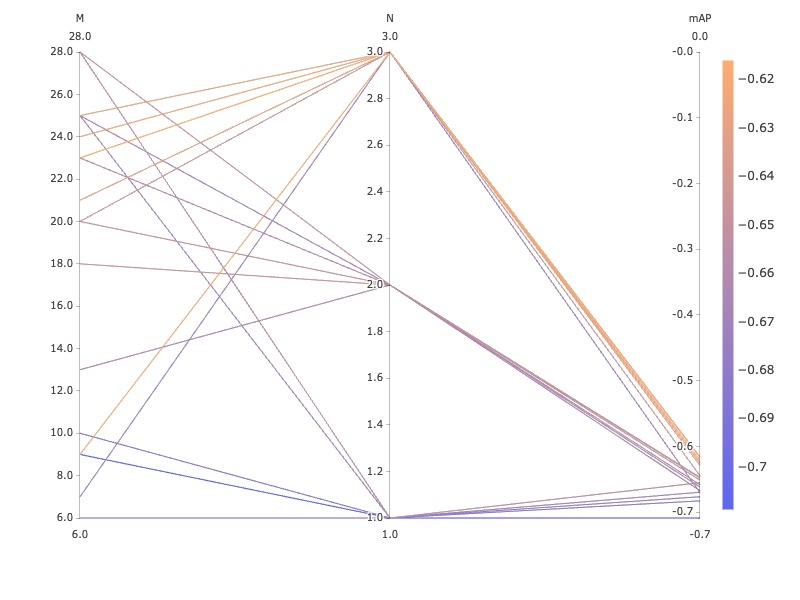
\includegraphics[width =0.90\textwidth]{images/graphic/mAP_ra_cars.jpeg}
        }
    \end{minipage}%
    \begin{minipage}{.5\linewidth}
        \centering
        \subfloat[Validation loss]{
            \label{RA_3:b}
            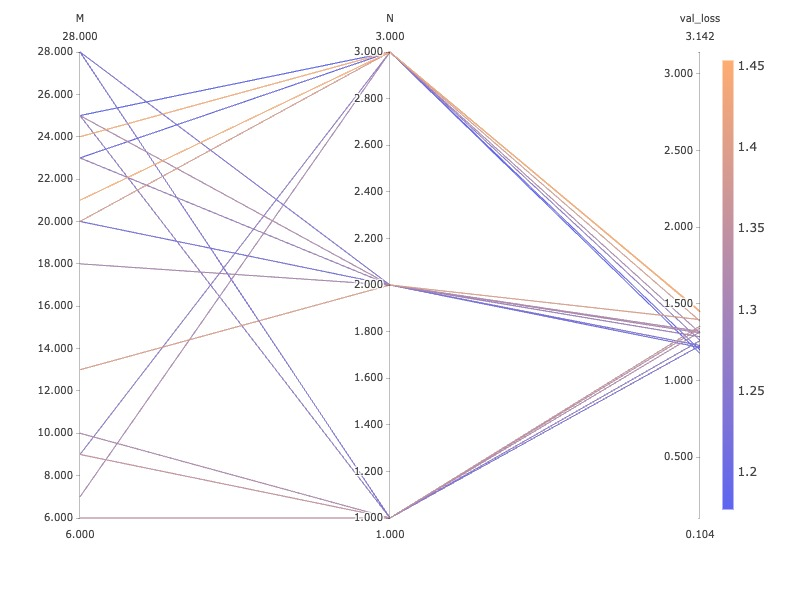
\includegraphics[width = 0.90\textwidth]{images/graphic/val_loss_ra_cars.jpeg}
            }
    \end{minipage}
    \begin{minipage}{.5\linewidth}
        \centering
        \subfloat[Risultati]{
            \label{RA_3:c}
            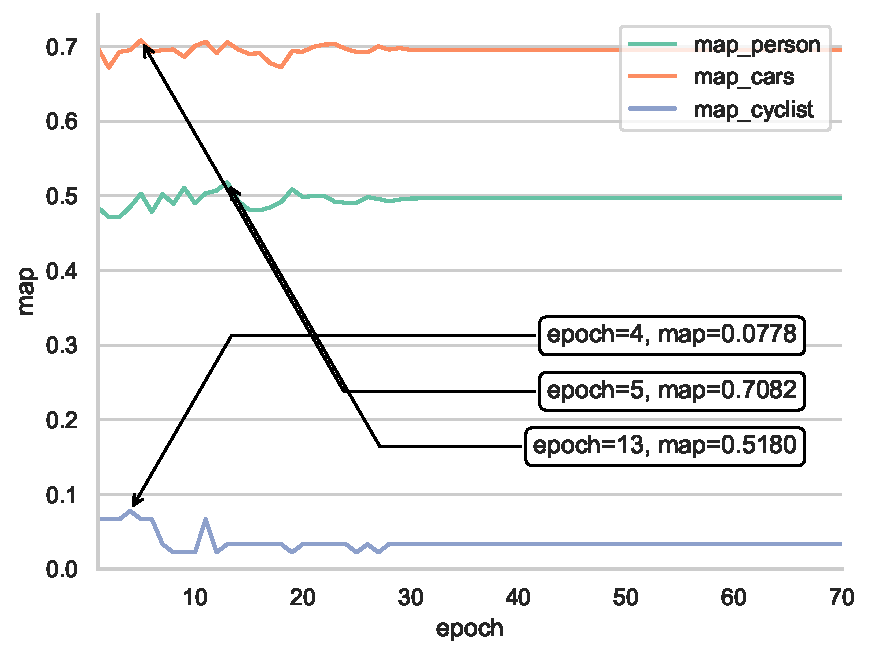
\includegraphics[width =0.90\textwidth]{images/graphic/graphics_map_ra_cars.pdf}
        }
    \end{minipage}%
    \centering
    \caption{Risultati ottenuti su \ac{kmpd} tramite l'ottimizzazione specifica di RandAugment su \texttt{cars}}
    \label{fig:RA_3}
\end{figure}


\paragraph{Generative Adversarial Network}
Con le \acf{GAN} si fa riferimento ad una classe di metodi basati su Reti Neurali introdotti da \textit{Ian Goodfellow} \cite{goodfellow2014generative} nel 2014 il cui scopo è generare nuovi dati. Scendendo un po' più nel dettaglio si hanno in particolare due reti che competono tra di loro: una rete generatrice $\mathcal{G}$ ed una rete discriminatrice $\mathcal{D}$. La rete $\mathcal{G}$, come si può intuire dal nome, si occupa di generare nuovi dati. La rete $\mathcal{D}$ invece si occupa di riconoscere dati reali da dati artificiali. Nvidia ha recentemente rilasciato \href{https://www.thispersondoesnotexist.com/}{un'applicazione web} \cite{Karras2019stylegan2} che facendo uso di \ac{GAN} genera volti di persone con risultati piuttosto impressionanti. 

Nel corso di questa tesi è stato fatto uso delle \ac{GAN} sulla parte di dataset di \ac{kmpd} annotatata con le vetture allo scopo di generare nuovi dati con cui addestrare RetinaNet. 
Partendo dalle immagini catturate dalle telecamere RGB sono state quindi generate immagini termiche del tutto realistiche ed utilizzabili per un'ulteriore fase di addestramento. In Figura \ref{fig:gan} è presente un'immagine tratta dal dataset \ac{kmpd} nelle sue tre varianti. La \ref{gan:a} è l'immagine nello spettro dei colori, mentre la \ref{gan:b} è la stessa immagine acquisita con telecamere termiche. La \ref{gan:c} è invece l'immagine generata con le \ac{GAN} partendo da \ref{gan:a}.
\begin{figure}[]
    \begin{minipage}{.29\linewidth}
        \centering
        \subfloat[RGB]{
            \label{gan:a}
            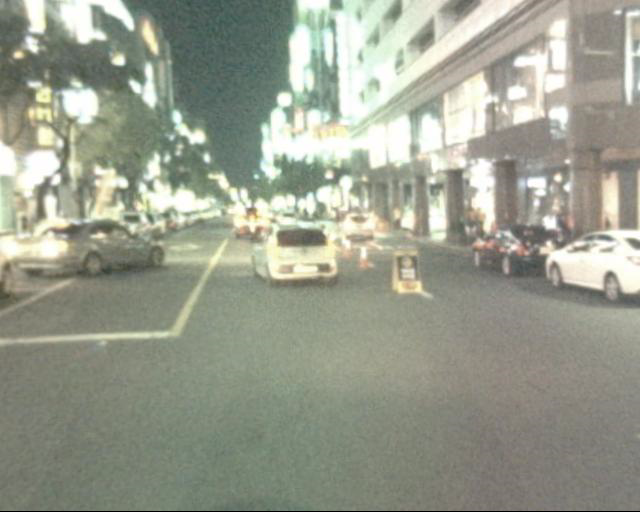
\includegraphics[width =0.90\textwidth]{images/examples/I00010_visible.jpg}
        }
    \end{minipage}%
    \begin{minipage}{.29\linewidth}
        \centering
        \subfloat[Termica]{
            \label{gan:b}
            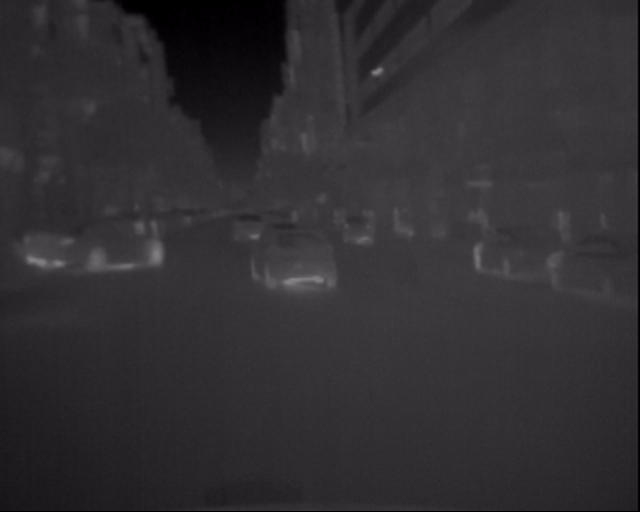
\includegraphics[width = 0.90\textwidth]{images/examples/I00010_lwir.jpg}
            }
    \end{minipage}
    \begin{minipage}{.29\linewidth}
        \centering
        \subfloat[GAN]{
            \label{gan:c}
            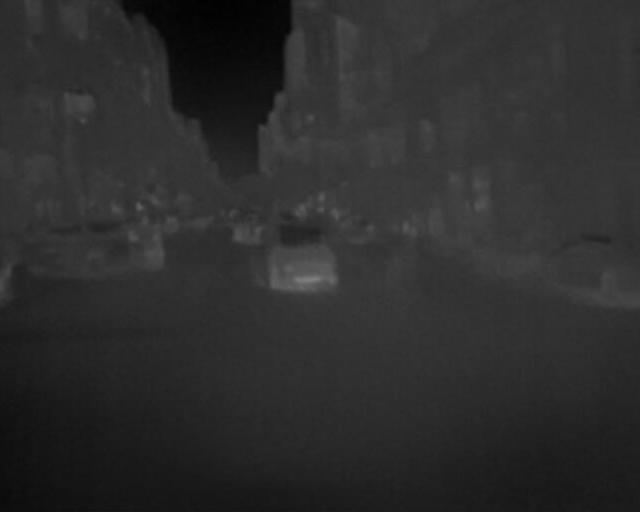
\includegraphics[width = 0.90\textwidth]{images/examples/I00010_gan.jpg}
            }
    \end{minipage}
    \centering
    \caption{Immagine di \ac{kmpd}}
    \label{fig:gan}
\end{figure}

Per realizzare questa forma di \textit{data augmentation} è stata utilizzata la parte di dataset di \ac{kmpd} su cui sono state annotate le vetture. Inizialmente si è proceduto con un addestramento di RetinaNet partendo da zero, vale a dire senza effettuare alcun tipo di transfer learning. 
I risultati ottenuti sono mostrati in Tabella \ref{tab:result_GAN_scratch} e come si può notare sono molto bassi, questo evidenzia che le tecniche di Data Augmentation vanno applicate a partire da una base solida per eventualmente aumentare le performance di un modello preaddestrato.

\begin{table}[]
    \resizebox{\textwidth}{!}{%
    \begin{tabular}{c|c|c|c|c|c|c|c|c|}
    \cline{2-9}
     & NOGAN & EP 1 & EP 5 & EP 10 & EP 15 & \textbf{EP 24} & \textbf{EP 27} & EP 30 \\ \hline
    \multicolumn{1}{|c|}{Person} & 0.1387 & 0.0086 & 0.1018 & 0.1344 & 0.1635 & 0.1767 & 0.1763 & 0.1817 \\ \hline
    \multicolumn{1}{|c|}{Cars} & 0.1358 & 0.1699 & 0.4014 & 0.3888 & 0.4086 & 0.4146 & 0.4573 & 0.4478 \\ \hline
    \end{tabular}}
    \caption{Risultati del test di RetinaNet sul dataset di \ac{kmpd} dopo una fase di addestramento su dati generati da \ac{GAN}. Nella colonna \textit{NOGAN} sono presenti i risultati ottenuti addestrando solamente sulla parte di \ac{kmpd} visibile e testando sul termico reale.}
    \label{tab:result_GAN_scratch}
\end{table}


Il risultato in Tabella \ref{tab:result_GAN_scratch} evidenzia come, attraverso un dataset generato da una \ac{GAN}, si ottengono risultati migliori rispetto ad avere solo il termico; considerato che i dataset termici sono molto pochi usare una \ac{GAN} per generare un dataset \textit{sintetico} è una valida alternativa.

Dopo questo esperimento il successivo è stato addestrare RetinaNet sulle immagini generate della \ac{GAN} partendo però dai pesi che ci hanno permesso di ottenere i risultati in Tabella \ref{tab:fine_tuning_kaist_flir}. I risultati di questa sperimentazione sono in Figura \ref{fig:fine_tuning_gan}, e come è possibile osservare non si ottiene alcuna miglioria, in nessuna delle classi. 
\begin{figure}[]
    \centering
    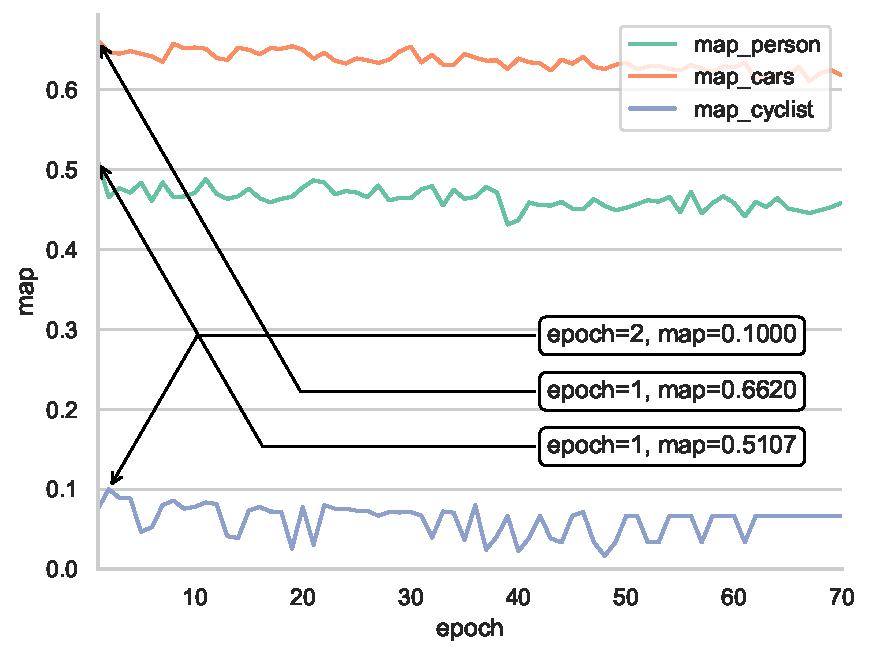
\includegraphics[width=\textwidth]{images/graphic/graphics_GAN.pdf}
    \caption{Risultati dopo fine tuning usando immagini genrate dalla GAN}
    \label{fig:fine_tuning_gan}
\end{figure}

\section{Esperimenti su video di RFI}
\label{sec:RFI_video_experiment}

I video termici di \ac{RFI} forniti sono tre, e su tutti e tre il task è la rilevazione di persone. Non essendo annotati la prima e unica operazione possibile è stata dare in pasto a RetinaNet i frame del video per realizzare inferenza usando i pesi migliori per la rilevazione di persone, ovvero quelli ottenuti tramite l'addestramento su \ac{kmpd} tramite la terza policy all'epoca 5 (Tabella \ref{table:aa_kaist}). 

I risultati iniziali appaiono promettenti benché da essi non si possano calcolare metriche, in quanto le rilevazioni sembrano abbastanza precise. 

I primi test sono stati effettuati tenendo una soglia di rilevazione pari a $0.30$, questo ha portato ad una rilevazione sempre accurata degli operai, ma anche a molte rilevazioni false, come ad esempio quelle mostrate in Figura \ref{fig:rfi_030}. 

\begin{figure}[]
    \begin{minipage}{.5\linewidth}
        \centering
        \subfloat[]{
            \label{rfi_030:a}
            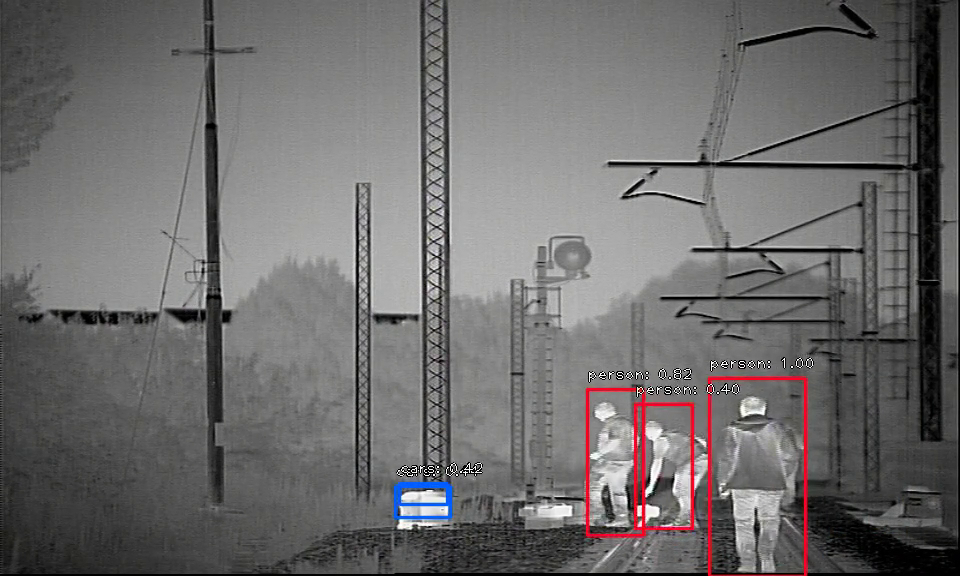
\includegraphics[width =0.99\textwidth]{images/examples/rfi_1_030_1.png}
        }
    \end{minipage}%
    \begin{minipage}{.5\linewidth}
        \centering
        \subfloat[]{
            \label{rfi_030:b}
            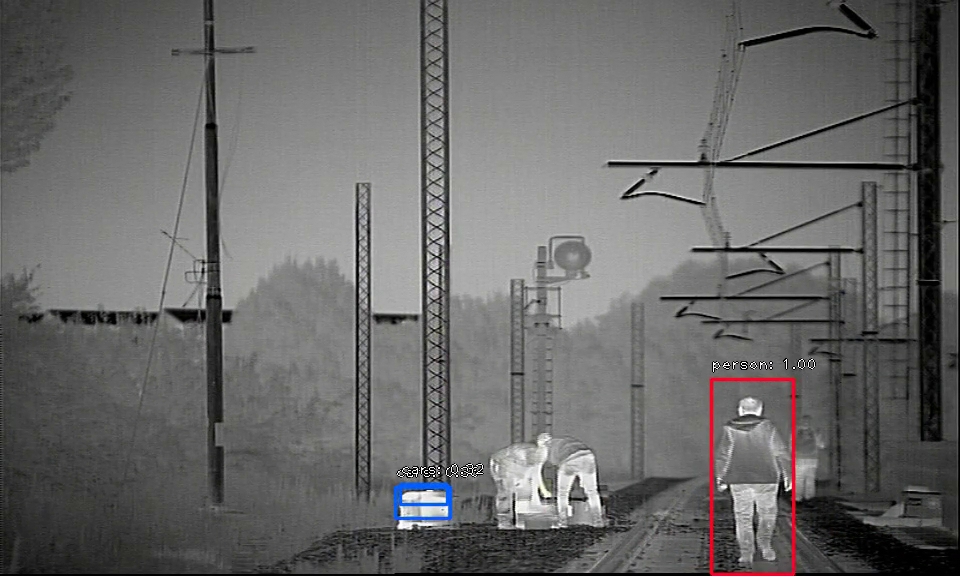
\includegraphics[width = 0.99\textwidth]{images/examples/rfi_1_030_2.png}
            }
    \end{minipage}
    \centering
    \caption{Rilevazioni su video RFI con soglia 0.30}
    \label{fig:rfi_030}
\end{figure}

Questo problema è facilmente risolvibile aumentando la soglia di rilevamento, infatti portandola a $0.8$ si rimuovono la maggior parte dei falsi positivi (Frame in Figura \ref{fig:rfi_080}). 

\begin{figure}[]
    \begin{minipage}{.5\linewidth}
        \centering
        \subfloat[]{
            \label{rfi_080:a}
            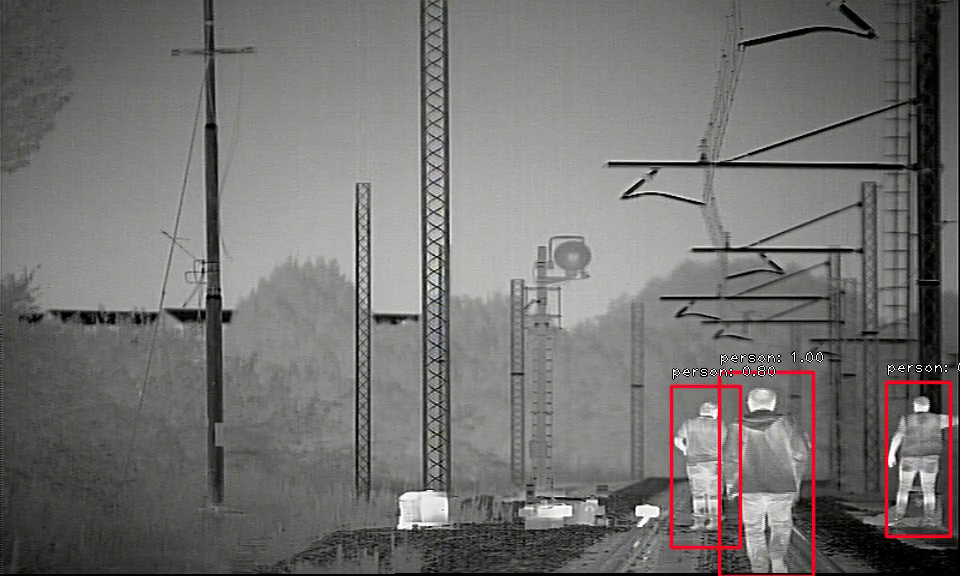
\includegraphics[width =0.99\textwidth]{images/examples/rfi_1_080_1.png}
        }
    \end{minipage}%
    \begin{minipage}{.5\linewidth}
        \centering
        \subfloat[]{
            \label{rfi_080:b}
            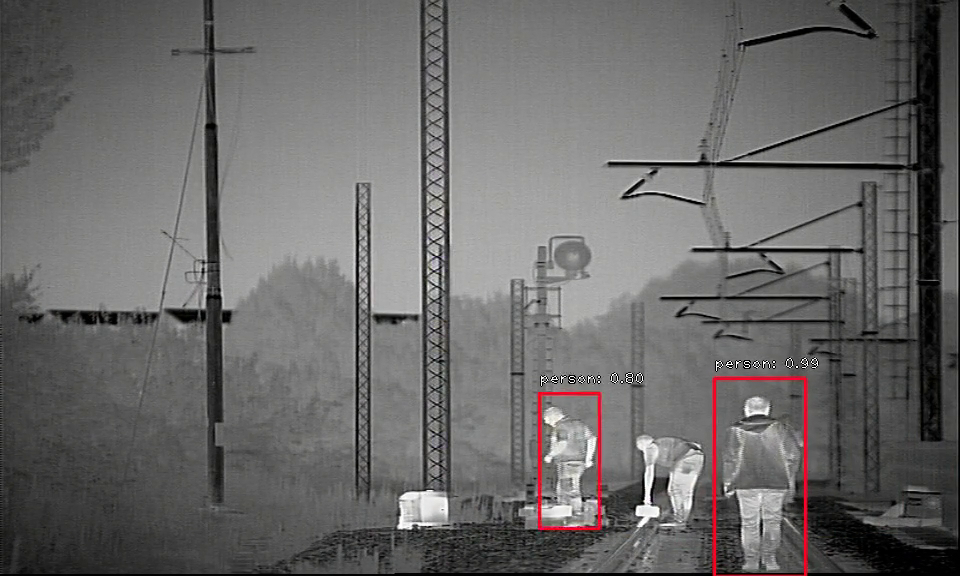
\includegraphics[width = 0.99\textwidth]{images/examples/rfi_1_080_2.png}
            }
    \end{minipage}
    \centering
    \caption{Rilevazioni su video RFI con soglia 0.80}
    \label{fig:rfi_080}
\end{figure}

Rimane però il problema  della rilevazione dei lavoratori in posizioni non usuali, ad esempio quando sono chinati. In Figura \ref{rfi_080:b} vi è un esempio in quanto l'operaio sembra stia raccogliendo qualcosa per terra e non è stato rilevato. Per risolvere il problema sono stati annotati alcuni frame di quel video per poi effettuare test su altri due video a nostra disposizione. 
\subsection{IoU sul tempo}
\label{sec:iou_over_time}
Allo scopo di ridurre ulteriormente il numero di falsi positivi all'interno dei video di \ac{RFI} è stato sviluppato un algoritmo che fa uso dell'indice di Jaccard (o \ac{IoU}) per validare le rilevazioni reali ed eliminare quelle fasulle. 
L'algoritmo in questione è in Algoritmo \ref{alg:iou}, mentre l'implementazione in Python è reperibile in Appendice \ref{appendix:a}.


\begin{algorithm}[H]
    \SetAlgoLined
    \SetKwInOut{Input}{Input}\SetKwInOut{Output}{Output}
    \Input{Detection di $N$ immagini, Threshold}
    \Output{Detection di $N$ immagini}
    \KwData{detections, T}
    \KwResult{detections'}
    $ max\_detections \leftarrow max\_detections\_in\_image(detections)$ \;
    $ R\_tree \leftarrow new\_r\_tree() $\;
    \For{$ d \in (detections - max\_detections)$}{
        $R\_tree.insert(d)$\;
    }
    $iou\_values \leftarrow empty\_array(len(max\_detections))$\;
    \For{$ d_i \in max\_detections$}{
        $intersected\_dets \leftarrow R\_tree.find\_intersection(d_i)$\;
        \For{$d_j \in intersected\_dets$} {
            $iou\_values[d_i] \text{ += } compute\_iou(d_i, d_j) $\;
        }
        $iou\_values[d_i] \text{ /= } len(intersected\_dets)$\; 
    }
    $detections' \leftarrow empty\_array(len(detections))$\;
    \For{$d_i \in max\_detections$}{
        \If{$iou\_values[d_i]>T$}{
            $detections'.insert(d_i)$\;
        }
    }
    \Return{$detections'$}
    \caption{Algoritmo di IoU calcolata su diversi frame}
    \label{alg:iou}
\end{algorithm}

L'input dell'algoritmo sono le rilevazioni effettuate su $N$ immagini ed una soglia $T$. 
Il primo passo effettuato è la ricerca dell'immagine contenente più rilevazioni in quanto è quella intuitivamente più soggetta ad avere qualche \ac{BB} trovata erroneamente durante la fase di inferenza, chiamiamola \textit{max\_detections}. Una volta trovata si inseriscono le detection di tutte le altre immagini all'interno di una struttura che ci permette di effettuare ricerche su coordinate spaziali in maniera efficiente, ovvero un albero R.

Dopodiché, presa l'immagine \textit{max\_detections}, si considerano singolarmente le \ac{BB} e si cercano attraverso l'albero R tutte le \ac{BB} nelle altre immagini che si intersecano alla singola \ac{BB} presa in esame, formando così un \textit{insieme intersezione}. 
Tramite queste \ac{BB} intersecanti si calcola un valore di \ac{IoU} tra la \ac{BB} presa in esame e tutte quelle nell'\textit{insieme intersezione}. Siccome la \ac{IoU} dev'essere un valore compreso tra $0$ e $1$, si normalizza usando il numero di frame $N$ in input.
Dopo questa fase avremo quindi un array di lunghezza pari al numero di \ac{BB} dell'immagine \textit{max\_detections} contenente valori di \ac{IoU}.
Nell'ultima parte dell'algoritmo si confronta ogni valore di questo array per vedere se è superiore alla soglia $T$ passata in input: se lo è la \ac{BB} corrispondente verrà inserita come detection \textit{valida} per ogni immagine nel batch, altrimenti viene scartata.

Come detto prima lo scopo finale dell'algoritmo non è tanto un miglioramento della \ac{map} generale tanto quanto la riduzione dei falsi positivi, ed applicando sui video forniti da \ac{RFI} nonostante non sia possibile calcolare metriche per via della mancanza di annotazioni si nota subito un miglioramento (Figura \ref{fig:alg_0} e \ref{fig:alg_1}).


\begin{figure}[]
    \begin{minipage}{.5\linewidth}
        \centering
        \subfloat[Prima]{
            \label{alg_0:a}
            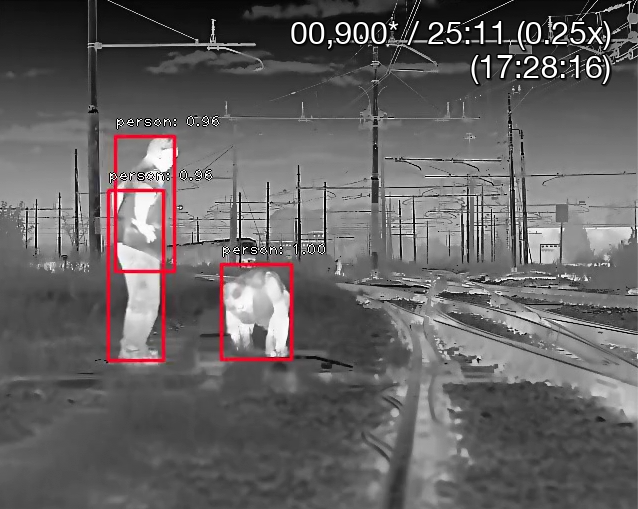
\includegraphics[width =0.99\textwidth]{images/examples/rfi_no_iou_0.png}
        }
    \end{minipage}%
    \begin{minipage}{.5\linewidth}
        \centering
        \subfloat[Dopo]{
            \label{alg_0:b}
            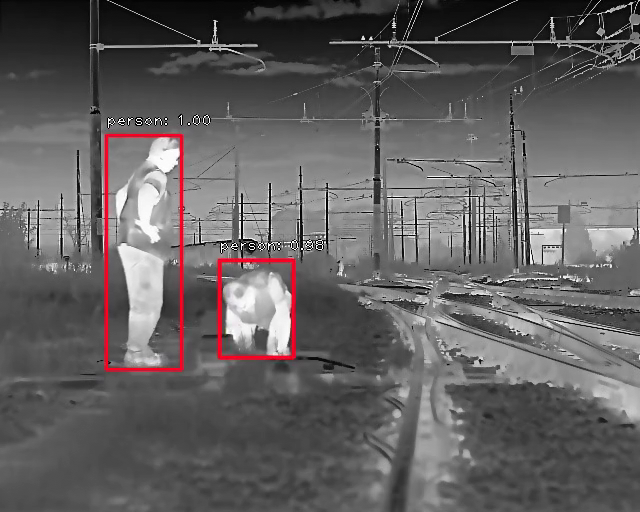
\includegraphics[width = 0.99\textwidth]{images/examples/rfi_iou_0.png}
            }
    \end{minipage}
    \centering
    \caption{Rilevazioni su video RFI con soglia 0.90, prima e dopo l'applicazione dell'algoritmo}
    \label{fig:alg_0}
\end{figure}
\begin{figure}[]
    \begin{minipage}{.5\linewidth}
        \centering
        \subfloat[Prima]{
            \label{alg_1:a}
            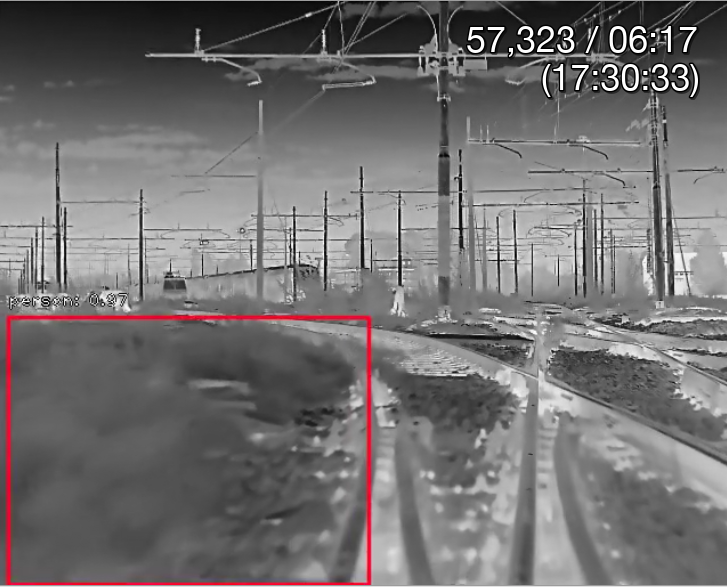
\includegraphics[width =0.99\textwidth]{images/examples/rfi_no_iou_1.png}
        }
    \end{minipage}%
    \begin{minipage}{.5\linewidth}
        \centering
        \subfloat[Dopo]{
            \label{alg_1:b}
            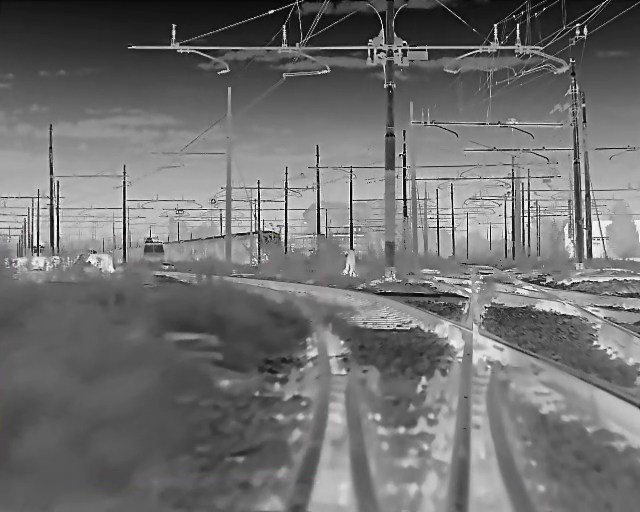
\includegraphics[width = 0.99\textwidth]{images/examples/rfi_iou_1.png}
            }
    \end{minipage}
    \centering
    \caption{Rilevazioni su video RFI con soglia 0.90, prima e dopo l'applicazione dell'algoritmo}
    \label{fig:alg_1}
\end{figure}